%\VignetteEngine{knitr::knitr}
%\VignetteIndexEntry{Integration of R and Scala Using rscala}

\documentclass[article]{jss}\usepackage[]{graphicx}\usepackage[]{color}
%% maxwidth is the original width if it is less than linewidth
%% otherwise use linewidth (to make sure the graphics do not exceed the margin)
\makeatletter
\def\maxwidth{ %
  \ifdim\Gin@nat@width>\linewidth
    \linewidth
  \else
    \Gin@nat@width
  \fi
}
\makeatother

\definecolor{fgcolor}{rgb}{0.345, 0.345, 0.345}
\newcommand{\hlnum}[1]{\textcolor[rgb]{0.686,0.059,0.569}{#1}}%
\newcommand{\hlstr}[1]{\textcolor[rgb]{0.192,0.494,0.8}{#1}}%
\newcommand{\hlcom}[1]{\textcolor[rgb]{0.678,0.584,0.686}{\textit{#1}}}%
\newcommand{\hlopt}[1]{\textcolor[rgb]{0,0,0}{#1}}%
\newcommand{\hlstd}[1]{\textcolor[rgb]{0.345,0.345,0.345}{#1}}%
\newcommand{\hlkwa}[1]{\textcolor[rgb]{0.161,0.373,0.58}{\textbf{#1}}}%
\newcommand{\hlkwb}[1]{\textcolor[rgb]{0.69,0.353,0.396}{#1}}%
\newcommand{\hlkwc}[1]{\textcolor[rgb]{0.333,0.667,0.333}{#1}}%
\newcommand{\hlkwd}[1]{\textcolor[rgb]{0.737,0.353,0.396}{\textbf{#1}}}%
\let\hlipl\hlkwb

\usepackage{framed}
\makeatletter
\newenvironment{kframe}{%
 \def\at@end@of@kframe{}%
 \ifinner\ifhmode%
  \def\at@end@of@kframe{\end{minipage}}%
  \begin{minipage}{\columnwidth}%
 \fi\fi%
 \def\FrameCommand##1{\hskip\@totalleftmargin \hskip-\fboxsep
 \colorbox{shadecolor}{##1}\hskip-\fboxsep
     % There is no \\@totalrightmargin, so:
     \hskip-\linewidth \hskip-\@totalleftmargin \hskip\columnwidth}%
 \MakeFramed {\advance\hsize-\width
   \@totalleftmargin\z@ \linewidth\hsize
   \@setminipage}}%
 {\par\unskip\endMakeFramed%
 \at@end@of@kframe}
\makeatother

\definecolor{shadecolor}{rgb}{.97, .97, .97}
\definecolor{messagecolor}{rgb}{0, 0, 0}
\definecolor{warningcolor}{rgb}{1, 0, 1}
\definecolor{errorcolor}{rgb}{1, 0, 0}
\newenvironment{knitrout}{}{} % an empty environment to be redefined in TeX

\let\hlesc\hlstd \let\hlpps\hlstd \let\hllin\hlstd \let\hlslc\hlcom \let\hlppc\hlcom
\usepackage{alltt}

\let\hlesc\hlstd \let\hlpps\hlstd \let\hllin\hlstd \let\hlslc\hlcom

\usepackage{lscape}
\usepackage{multicol}
\usepackage{multirow}
\usepackage{rotating}
\usepackage{booktabs}
\usepackage{paralist}
\usepackage{thumbpdf}
\usepackage[11pt]{moresize}
\usepackage{alltt}
\usepackage{amsmath}
\usepackage{textcomp}
\usepackage[T1]{fontenc}
\setcounter{secnumdepth}{3}
\setcounter{tocdepth}{3}
%\overfullrule=3mm
\usepackage{fancyvrb}

%%%%%%%%%%%%%%%%%%%%%%%%%%%%%%
%% declarations for jss.cls %%
%%%%%%%%%%%%%%%%%%%%%%%%%%%%%%

\usepackage{xspace}

\newcommand{\rscala}{\pkg{rscala}\xspace}
\newcommand{\jvmr}{\pkg{jvmr}\xspace}
\newcommand{\rJava}{\pkg{rJava}\xspace}
\newcommand{\Rserve}{\pkg{Rserve}\xspace}
\newcommand{\Rcpp}{\pkg{Rcpp}\xspace}
\newcommand{\inline}{\pkg{Inline}\xspace}
\newcommand{\R}{\proglang{R}\xspace}
\newcommand{\Rscript}{\proglang{Rscript}\xspace}
\newcommand{\C}{\proglang{C}\xspace}
\newcommand{\Python}{\proglang{Python}\xspace}
\newcommand{\Csharp}{\proglang{C\#}\xspace}
\newcommand{\Ruby}{\proglang{Ruby}\xspace}
\newcommand{\Cpp}{\proglang{C++}\xspace}
\newcommand{\Scala}{\proglang{Scala}\xspace}
\newcommand{\Java}{\proglang{Java}\xspace}
\newcommand{\Fortran}{\proglang{Fortran}\xspace}
\newcommand{\BeanShell}{\pkg{BeanShell}\xspace}
\newcommand{\todo}[1]{\textbf{\textit{\colorbox{yellow}{\color{red}{TODO} \ldots #1}}}}

%% almost as usual
\author{David B.\ Dahl\\Brigham Young University}
\title{\textit{\Large Under Review\\\footnotesize Software Version: 3.2.0-SNAPSHOT,\ \ Document ID: 2018-07-30}\\\vspace{5ex} Integration of \R and \Scala Using \rscala}

%% for pretty printing and a nice hypersummary also set:
\Plainauthor{David B. Dahl} %% comma-separated
\Plaintitle{Integration of R and Scala Using rscala} %% without formatting
\Shorttitle{Integration of \R and \Scala Using \rscala} %% a short title (if necessary)

%% an abstract and keywords
\Abstract{
The \rscala software is a simple, two-way bridge between \R and \Scala that
allows users to leverage the unique strengths of both languages in a
single project.  \Scala classes can be instantiated from \R and \Scala methods
can be called.  Arbitrary \Scala code can be executed on-the-fly from within
\R, inline \Scala functions can be defined, and callbacks to \R are supported.
\R packages can be developed using \Scala.  Conversely, \rscala also enables \R
code to be embedded within a \Scala application.  The \rscala package is
available on CRAN and has no dependencies beyond base \R and the \Scala
standard library.
}

\Keywords{Java Virtual Machine, JVM, language bridges, \R, \Scala}
\Plainkeywords{Java Virtual Machine, JVM, language bridges, R, Scala} %% without formatting

%% at least one keyword must be supplied

%% publication information
%% NOTE: Typically, this can be left commented and will be filled out by the technical editor
%% \Volume{50}
%% \Issue{9}
%% \Month{June}
%% \Year{2012}
\Submitdate{2017-08-22}
%% \Acceptdate{2012-06-04}

%% The address of (at least) one author should be given
%% in the following format:
\Address{
  David B.\ Dahl\\
  Professor\\ % and Associate Department Chair\\
  Department of Statistics\\
  Brigham Young University \\
  223 TMCB\\
  Provo, UT 84602\\
  E-mail: \email{dahl@stat.byu.edu}\\
  URL: \url{https://dahl.byu.edu}\\
}

%% It is also possible to add a telephone and fax number
%% before the e-mail in the following format:
%% Telephone: +43/512/507-7103
%% Fax: +43/512/507-2851

%% for those who use Sweave please include the following line (with % symbols):
%% need no \usepackage{Sweave.sty}

%% end of declarations %%%%%%%%%%%%%%%%%%%%%%%%%%%%%%%%%%%%%%%%%%%%%%%

%% \renewcommand{\textfraction}{0.05}
%% \renewcommand{\topfraction}{0.95}
%% \renewcommand{\bottomfraction}{0.95}
%% \renewcommand{\floatpagefraction}{0.35}
%% \setcounter{totalnumber}{5}
\IfFileExists{upquote.sty}{\usepackage{upquote}}{}
\begin{document}

% Fix poorly formatted tilde.
\newcommand{\mytilde}{\lower.6ex\hbox{\char`\~}}


%% include your article here, just as usual
%% Note that you should use the \pkg{}, \proglang{} and \code{} commands.

\section{Introduction}
\label{introduction}

This paper introduces \rscala \citep{rscala}, software that provides a bridge
between \R \citep{r} and \Scala \citep{scala}.  The goal of \rscala is to allow
users to leverage the unique strengths of \Scala and \R in a single program.
For example, \R packages can implement computationally-intensive algorithms in
\Scala and, conversely, \Scala applications can take advantage of the vast
array of statistical packages in \R.  Callbacks from embedded \Scala into \R
are supported.  The \rscala package is available on the Comprehensive \R
Archive Network (CRAN).  Also, \R can be embedded within a \Scala application
by adding a one-line dependency declaration in \pkg{Scala Build Tool} (SBT).

\Scala is a general-purpose programming language that is designed to strike a
balance between execution speed and programmer productivity.  \Scala programs
run on the Java Virtual Machine (JVM) at speeds comparable to \Java.  \Scala
features object-oriented, functional, and imperative programming paradigms,
affording developers flexibility in application design.  \Scala code can be
concise, thanks in part to type inference, higher-order functions, multiple
inheritance through traits, and a large collection of libraries.  \Scala also
supports pattern matching, operator overloading, optional and named parameters,
and string interpolation. \Scala encourages immutable data types and pure
functions (i.e., functions without side-effects) to simplify parallel
processing and unit testing. In short, the \Scala language implements many of
the most productive ideas in modern computing. To learn more about \Scala, we
suggest \emph{Programming in Scala} \citep{scalabook} as an excellent general
reference.

Because \Scala is flexible, concise, and quick to execute, it is emerging as an
important tool for scientific computing. For example, \pkg{Spark} \citep{spark}
is a cluster-computing framework for massive datasets written in \Scala.
Several books have been published recently on using \Scala for data science
\citep{a9781785281372}, scientific computing \citep{a9781785886942}, machine
learning \citep{a9781783558742}, and probabilistic programming
\citep{a9781617292330}.  We believe that \Scala deserves consideration when
looking for an efficient and convenient general-purpose programming language to
complement \R.

\R is a scripting language and environment developed by statisticians for
statistical computing and graphics.  Like \Scala, \R supports a functional
programming style and provides immutable data types.  \Scala programmers who
learn \R (and vice versa) will find many familiar concepts, despite the
syntactical differences.  \R has a massive user base of statisticians and over
11,000 actively-maintained packages on CRAN. Hence, the \Scala community has a
lot to gain from an integration with \R.

\R code can be very concise and expressive, but may run significantly slower
than compiled languages.  In fact, computationally intensive algorithms in \R
are typically implemented in compiled languages such as \C, \Cpp, \Fortran, and
\Java. The \rscala package adds \Scala to this list of high-performance
languages that can be used to write \R extensions. The \rscala package is
similar in concept to \Rcpp \citep{rcpp}, an \R integration for \C and \Cpp,
and \rJava \citep{rJava}, an \R integration for \Java. Though the \rscala
integration is not as comprehensive as \Rcpp and \rJava, it provides the
following important features to blend \R and \Scala.  First, \rscala allows
arbitrary \Scala snippets to be included within an \R script and \Scala objects
can be created and referenced directly within \R code. These features allow
users to integrate \Scala solutions in an existing \R workflow.  Second,
\rscala supports callbacks to \R from \Scala, which allow developers to
implement general, high-performance algorithms in \Scala (e.g., root finding
methods) based on user-supplied \R functions.  Third, \rscala supports
developing \R packages based on \Scala which allows \Scala developers to make
their work available to the \R community.  Finally, the \rscala software makes
it easy to incorporate \R in a \Scala application without even having to install
the \R package.  In sum, \rscala's feature-set makes it easy to exploit the
strengths of \R and \Scala in a single project.

We now discuss the implementation of \rscala and some relevant existing work.
Since \Scala code compiles to \Java byte code and runs on the JVM, one could
access \Scala from \R via \rJava and then benefit from the speed of shared
memory.  We originally implemented our \rscala bridge using this technique, but
later moved to a custom TCP/IP protocol for the following reasons.  First,
\rJava and \Scala's read-eval-print loop (REPL) are both implemented using
custom class loaders which, in our experience, conflict with each other in some
cases.  Second, since \rJava links to a single instance of the JVM, one
\rJava-based package can configure the JVM in a manner that is not compatible
with a second \rJava-based package.  The current \rscala package creates a new
instance of the JVM for each \Scala instance to avoid such conflicts.  Third,
the simplicity of no dependencies beyond \Scala's standard library and base \R
is appealing from a user's perspective.  Finally, callbacks in \rJava are
provided by the optional JRI component, which is only available if \R is built
as a shared library.  While this is the case on many platforms, it is not
universal and therefore callbacks could not be a guaranteed feature of \rscala
software if it were based on \rJava's JRI.

The discussion of the design of \rscala has so far focused on accessing \Scala
from \R.  The \rscala software also supports accessing \R from \Scala using the
same TCP/IP protocol.  This ability is an offshoot of the callback
functionality.  Since \Scala can call \Java libraries, those who are interested
in accessing \R from \Scala should also consider the \Java libraries \Rserve
\citep{rserve} and \pkg{RCaller} \citep{rcaller}.  \Rserve is also ``a TCP/IP
server which allows other programs to use facilities of \R''
(\url{http://www.rforge.net/Rserve}).  \Rserve clients are available for many
languages including \Java.  \Rserve is fast and provides a much richer API than
\rscala.  Like \rJava, however, \Rserve also requires that \R be compiled as a
shared library.  Also, Windows has some limitations such that \Rserve users are
advised not to ``use Windows unless you really have to''
(\url{http://www.rforge.net/Rserve/doc.html}).

The paper is organized as follows.  Section \ref{scalainr} describes using
\Scala from \R.  Some of the more important topics presented there include the
data types supported by \rscala, embedding \Scala snippets in an \R script,
accessing precompiled \Scala code from \R, defining inline \Scala functions,
and calling back into \R from embedded \Scala.  We also discuss how to develop
\R packages based on \Scala.  Section \ref{rinscala} describes using \R from
\Scala.  In both Sections\ \ref{scalainr} and \ref{rinscala}, concise examples
are provided to help describe the software's functionality.  Section
\ref{bootstrap} provides a case study to show how \Scala can easily be embedded
in \R to significantly reduce computation time for a simulation study.  We
conclude in Section \ref{conclusion} with future work.

\section[Accessing Scala in R]{Accessing \Scala in \R}
\label{scalainr}

This section provides a guide to accessing
\Scala from \R.  Those interested in the reverse --- accessing \R from \Scala
--- will also benefit from understanding the ideas presented here.

\subsection[Package and Scala installation]{Package and \Scala installation}

The \rscala package is available on the Comprehensive \R Archive Network (CRAN)
and can be installed by executing the following \R expression.

\begin{knitrout}\small
\definecolor{shadecolor}{rgb}{0.969, 0.969, 0.969}\color{fgcolor}\begin{kframe}
\begin{alltt}
\hlkwd{install.packages}\hlstd{(}\hlstr{'rscala'}\hlstd{)}
\end{alltt}
\end{kframe}
\end{knitrout}

The \rscala package requires a \Scala installation in the 2.11.x or
2.12.x series.  A convenience function, \code{rscala::scalaInstall()}, is
provided to download and install \Scala in the user's home directory under the
\code{.rscala} directory. Because this is a user-level installation,
administrator privileges are not required.
System administrators can execute \code{rscala::scalaInstall(global=TRUE)},
which places Scala in the package's directory but requires a new installation
every time the package is updated.  To avoid this, system administrators can
install \Scala using their operating system's software management system (e.g.,
``\code{sudo apt install scala}'' on Debian/Ubuntu based systems).  Finally,
both administrators and users can use a manual installation as described on the
\Scala webpage.

\subsection[Instantiating a Scala interpreter in R]{Instantiating a \Scala interpreter in \R}

Load and attach the \rscala package in an \R session with the \code{library} function:

\begin{knitrout}\small
\definecolor{shadecolor}{rgb}{0.969, 0.969, 0.969}\color{fgcolor}\begin{kframe}
\begin{alltt}
\hlkwd{library}\hlstd{(}\hlstr{'rscala'}\hlstd{)}
\end{alltt}
\end{kframe}
\end{knitrout}

Create a \Scala instance using the \code{scala} function:

\begin{knitrout}\small
\definecolor{shadecolor}{rgb}{0.969, 0.969, 0.969}\color{fgcolor}\begin{kframe}
\begin{alltt}
\hlkwd{scala}\hlstd{()}
\end{alltt}
\end{kframe}
\end{knitrout}



This implicitly makes the interpreter instance \code{s} available in the current
environment.  (The name can be customized with the \code{assign.name} option of the \code{scala} function.)
Information on the \Scala instance \code{s} is available using

\begin{knitrout}\small
\definecolor{shadecolor}{rgb}{0.969, 0.969, 0.969}\color{fgcolor}\begin{kframe}
\begin{alltt}
\hlkwd{scalaInfo}\hlstd{()}
\end{alltt}
\end{kframe}
\end{knitrout}

Alternatively, details on the search for a suitable \Scala installation are
shown using

\begin{knitrout}\small
\definecolor{shadecolor}{rgb}{0.969, 0.969, 0.969}\color{fgcolor}\begin{kframe}
\begin{alltt}
\hlkwd{scalaInfo}\hlstd{(}\hlkwc{verbose}\hlstd{=}\hlnum{TRUE}\hlstd{)}
\end{alltt}
\end{kframe}
\end{knitrout}

The \code{scala} function includes parameters to specify which \Scala
installation to use, the class path, whether matrices are in row-major or
column-major order, and several other settings.  The functions \code{scala2}
and \code{scala3} are equivalent to \code{scala} except they change the \code{mode}
option to customize how the bridge between \Scala and \R is established.
Interactive users may notice that the \code{scala} function feels faster because
it starts \Scala in the background.  Details on this and all
other functions are provided in the \R documentation for the package (e.g.,
\code{help(scala)}).

A \Scala session is only valid during the \R session in which it is created and
cannot be saved and restored through, for example, the \code{save} and
\code{load} functions.  Multiple \Scala instances can be created in the same \R
session.  Each \Scala instance runs independently with its own memory and
classpath.

The \R to \Scala bridge is not thread-safe so multiple \R processes/threads
should not access the same \Scala instance simultaneously.

\subsection[Calling Scala code from R]{Calling \Scala code from \R}

\subsubsection[Evaluating Scala snippets]{Evaluating \Scala snippets}

Snippets of \Scala code can be compiled and executed within an \R session using
several operators.  The most basic operator is \code{\%@\%} which evaluates
\Scala code and returns \code{NULL}.  Consider, for example, computing the
binomial coefficient ${10 \choose 3} = \prod_{i=1}^3 (10-i+1)/i$.  The code below
uses \Scala's \code{val} statement to define an immutable variable
\code{c_10_3}.  The expression \code{1 to 3} creates a range and the higher-order \code{map} method of the
range applies the function \code{(10-i+1) / i.toDouble} to each element \code{i} in the range.
Finally, the results are multiplied together by the \code{product} method.

\begin{knitrout}\small
\definecolor{shadecolor}{rgb}{0.969, 0.969, 0.969}\color{fgcolor}\begin{kframe}
\begin{alltt}
\hlstd{s} \hlopt{+} \hlstr{'
  val c_10_3 = (1 to 3).map( i => \{
    (10-i+1) / i.toDouble
  \}).product.toInt
'}
\end{alltt}
\begin{verbatim}
## NULL
\end{verbatim}
\end{kframe}
\end{knitrout}

This result is available in subsequent \Scala expressions as demonstrated
below.

\begin{knitrout}\small
\definecolor{shadecolor}{rgb}{0.969, 0.969, 0.969}\color{fgcolor}\begin{kframe}
\begin{alltt}
\hlstd{s} \hlopt{*} \hlstr{'print("10 choose 3 is " + c_10_3 + ".")'}
\end{alltt}
\begin{verbatim}
## 10 choose 3 is 120.
## NULL
\end{verbatim}
\end{kframe}
\end{knitrout}

Notice the side effect of printing \code{120} to the console.  The behavior for
console printing is controlled by the arguments \code{serialize.output},
\code{stdout}, and \code{stderr} of the \code{scala} function.  Default values
depend on the operating system and are set such that console output is
displayed in typical environments.

\Scala snippets can also be evaluated with the \code{\%\mytilde\%} operator.
Whereas \code{\%@\%} always returns \code{NULL}, \code{\%\mytilde\%} returns
the result of the last expression in the \Scala snippet.

\begin{knitrout}\small
\definecolor{shadecolor}{rgb}{0.969, 0.969, 0.969}\color{fgcolor}\begin{kframe}
\begin{alltt}
\hlstd{tenChooseThree} \hlkwb{<-} \hlstd{s} \hlopt{*} \hlstr{'(1 to 3).map( i => (10-i+1) / i.toDouble ).product'}
\hlstd{tenChooseThree} \hlopt{==} \hlkwd{choose}\hlstd{(}\hlnum{10}\hlstd{,}\hlnum{3}\hlstd{)}
\end{alltt}
\begin{verbatim}
## [1] TRUE
\end{verbatim}
\end{kframe}
\end{knitrout}

\subsubsection{String interpolation}

The \rscala package features string interpolation for dynamic code snippets. \R
code placed between ``\code{@\{}'' and ``\code{\}}'' in a \Scala snippet is
evaluated and replaced by the string representation of the \R expression's
value before the \Scala snippet is executed. The \R code is executed in the
same environment (i.e., scope) as the evaluation request. A snippet can contain
any number of \code{@\{...\}} expressions.  For example,

\begin{knitrout}\small
\definecolor{shadecolor}{rgb}{0.969, 0.969, 0.969}\color{fgcolor}\begin{kframe}
\begin{alltt}
\hlstd{n} \hlkwb{<-} \hlnum{10L}
\hlstd{k} \hlkwb{<-} \hlnum{3L}
\hlstd{label} \hlkwb{<-} \hlstr{"number of threesomes among ten people"}
\hlstd{count} \hlkwb{<-} \hlkwd{s}\hlstd{(n,k,label)} \hlopt{*} \hlstr{'
  val count = (1 to k).foldLeft(1) \{ (prod,i) => prod * (n-i+1)/i \}
  println(s"The $label is $count.")
  count
'}
\end{alltt}
\begin{verbatim}
## The number of threesomes among ten people is 120.
\end{verbatim}
\end{kframe}
\end{knitrout}

Care is needed when using string interpolation because it relies on \R's
character representation on an \R expression.  One might be surprised, for
example, that the second expression in the next example is false. This is
because \code{@\{tenChooseThree\^{}20\}} is replaced by \code{6.191736e+20}
which, when parsed by the Scala compiler, leads to a slightly different value
than the calculated value.

\begin{knitrout}\small
\definecolor{shadecolor}{rgb}{0.969, 0.969, 0.969}\color{fgcolor}\begin{kframe}
\begin{alltt}
\hlkwd{s}\hlstd{(}\hlkwc{tenChooseThreePow20}\hlstd{=count}\hlopt{^}\hlnum{20}\hlstd{,count)} \hlopt{*} \hlstr{'math.pow(count, 20) == tenChooseThreePow20'}
\end{alltt}
\begin{verbatim}
## [1] TRUE
\end{verbatim}
\end{kframe}
\end{knitrout}

\subsubsection{Primitive and copyable types}

A \Scala result of class \code{Byte}, \code{Int}, \code{Double},
\code{Boolean}, or \code{String} is passed back to \R as a length-one vector of
raw, integer, double, logical, or character, respectively.  We refer to these
as the \emph{primitive types} supported by the \rscala package. Further, \Scala
arrays and rectangular arrays of arrays of the primitive types are passed to \R
as vectors and matrices of the equivalent \R types.  We call \emph{copyable
types} those types that are primitives, arrays of primitives, and rectangular
arrays of arrays of the primitive types.  The name emphasizes the fact that
these data structures are serialized and copied between \Scala and \R. This may
be a costly exercise for large data structures.

The code below produces a 2x5 matrix in \R.  If the \code{row.major} argument
of the \code{scala} function is changed to \code{FALSE} when defining the
\Scala instance \code{s}, the code produces a 5x2 matrix instead.

\begin{knitrout}\small
\definecolor{shadecolor}{rgb}{0.969, 0.969, 0.969}\color{fgcolor}\begin{kframe}
\begin{alltt}
\hlstd{s} \hlopt{*} \hlstr{'Array.fill(2)(Array.fill(5)(scala.util.Random.nextDouble))'}
\end{alltt}
\begin{verbatim}
##           [,1]      [,2]      [,3]      [,4]      [,5]
## [1,] 0.1295506 0.1869817 0.2251667 0.4842633 0.6471656
## [2,] 0.6973052 0.7649155 0.6072049 0.9374167 0.5987982
\end{verbatim}
\end{kframe}
\end{knitrout}

Table \ref{mappings} shows the mapping of primitive \Scala and \R types using
code examples.

\begin{table}[tb]
\scriptsize
\centering
\begin{tabular}{lll}
\toprule
     \textbf{Primitives} & \textbf{Vectors / Arrays} & \textbf{Matrices / Rectangular Arrays of Arrays} \\
\midrule
\noalign{\vspace{2ex}}
\code{a <- as.raw(3)} & \code{f <- as.raw(c(1, 2))} & \code{k <- matrix(as.raw(c(1, 2)), nrow=2)} \\
\code{val a = 3.toByte} & \code{val f = Array(1.toByte, 2.toByte)} & \code{val k = Array(Array(1.toByte), Array(2.toByte))} \\
\noalign{\vspace{4ex}}
\code{b <- TRUE} & \code{g <- c(TRUE, FALSE)} & \code{l <- matrix(c(TRUE, FALSE), nrow=2)} \\
\code{val b = true} & \code{val g = Array(true, false)} & \code{val l = Array(Array(true), Array(false))} \\
\noalign{\vspace{4ex}}
 \code{c <- 1L} & \code{h <- c(1L, 2L, 3L)} & \code{m <- matrix(c(1L, 2L), nrow=2)} \\
 \code{val c = 1} & \code{val h = Array(1, 2, 3)} & \code{val m = Array(Array(1), Array(2))} \\
\noalign{\vspace{4ex}}
 \code{d <- 1.0} & \code{i <- c(1.0, 2.0, 3.0)} & \code{n <- matrix(c(1.0, 2.0), nrow=2)} \\
 \code{val d = 1.0} & \code{val i = Array(1.0, 2.0, 3.0)} & \code{val n = Array(Array(1.0), Array(2.0))} \\
\noalign{\vspace{4ex}}
 \code{e <- "a"} & \code{j <- c("a", "b", "c")} & \code{o <- matrix(c("a", "b"), nrow=2)} \\
 \code{val e = "a"} & \code{val j = Array("a", "b", "c")} & \code{val o = Array(Array("a"), Array("b"))} \\
\noalign{\vspace{2ex}}
\bottomrule
\end{tabular}
\caption{\Scala values of type \code{Byte}, \code{Int}, \code{Double},
\code{Boolean}, or \code{String} (labeled \emph{primitives}), as well as arrays
and rectangular arrays of arrays of these types are copied from \Scala to \R as
length-one vectors, vectors, and matrices of the equivalent \R types.  These
are called \emph{copyable types}.  Each cell in the table contains two lines:
an \R expression (top) and the equivalent \Scala expression (bottom) with the
same identifier.  The matrix examples assume that the \code{scala} function is
called with \code{row.major=TRUE}.}
\label{mappings}
\end{table}

\subsubsection[Scala references]{\Scala references}

If the result of a \Scala expression is not a copyable type, then the
\code{\%\mytilde\%} operator will return a reference to a \Scala object that
can be used in subsequent evaluations.  If a \Scala reference is desired, even
when working with copyable types, use the \code{\%.\mytilde\%} operator.

In the next example, an instance of the class \code{scala.util.Random} is
created and, because the result is not a copyable type, a \Scala reference is
returned.  Second, a \Scala reference to an array of integers is returned,
despite the fact this is a copyable type, because the \code{\%.\mytilde\%}
operator is used.

\begin{knitrout}\small
\definecolor{shadecolor}{rgb}{0.969, 0.969, 0.969}\color{fgcolor}\begin{kframe}
\begin{alltt}
\hlstd{rng} \hlkwb{<-} \hlstd{s} \hlopt{*} \hlstr{'new scala.util.Random()'}
\hlstd{rng}
\end{alltt}
\begin{verbatim}
## rscala reference of type scala.util.Random
\end{verbatim}
\begin{alltt}
\hlstd{oneToTenReference} \hlkwb{<-} \hlstd{s} \hlopt{^} \hlstr{'Array.range(1,11)'}
\hlstd{oneToTenReference}
\end{alltt}
\begin{verbatim}
## rscala reference of type Array[Int]
\end{verbatim}
\end{kframe}
\end{knitrout}

% In the next example, a \Scala reference is used via string interpolation to
% call methods of \Scala objects:
% 
% \clearpage
% <<evaluateScalaCodeReferenceInterpolation>>=
% s * '
%   @{rng}.setSeed(24234)
%   @{rng}.nextDouble()
% '
% 
% s * '@{oneToTenReference}.sum'
% @

\subsubsection{Getting and setting variables}

Values of copyable types and \Scala references can be obtained as the result of
evaluating a \Scala expression using the \code{\%\mytilde\%} and
\code{\%.\mytilde\%} operators.  The expression can be very complex or, as in
the examples below, merely the name of a \Scala identifier.

\begin{knitrout}\small
\definecolor{shadecolor}{rgb}{0.969, 0.969, 0.969}\color{fgcolor}\begin{kframe}
\begin{alltt}
\hlstd{s} \hlopt \hlstr{'val fibSeq = Array[Double](0, 1, 1, 2, 3, 5, 8, 13, 21)'}
\end{alltt}


{\ttfamily\noindent\bfseries\color{errorcolor}{\#\# Error in s \%@\% "{}val fibSeq = Array[Double](0, 1, 1, 2, 3, 5, 8, 13, 21)"{}: could not find function "{}\%@\%"{}}}\begin{alltt}
\hlstd{fibSeqAsDouble}  \hlkwb{<-} \hlstd{s} \hlopt{*}  \hlstr{'fibSeq'}
\end{alltt}
\begin{verbatim}
## <console>:13: error: not found: value fibSeq
##        fibSeq
##        ^
\end{verbatim}


{\ttfamily\noindent\bfseries\color{errorcolor}{\#\# Error in pop(details, transcompileInfo, envir): Compilation error. Code is:\\\#\# () => \{\\\#\# fibSeq\\\#\# \}}}\begin{alltt}
\hlstd{fibSeqReference} \hlkwb{<-} \hlstd{s} \hlopt{^} \hlstr{'fibSeq'}
\end{alltt}
\begin{verbatim}
## <console>:13: error: not found: value fibSeq
##        fibSeq
##        ^
\end{verbatim}


{\ttfamily\noindent\bfseries\color{errorcolor}{\#\# Error in pop(details, transcompileInfo, envir): Compilation error. Code is:\\\#\# () => \{\\\#\# fibSeq\\\#\# \}}}\end{kframe}
\end{knitrout}

\Scala values can also be obtained using the \code{\$} operator and the
identifier name.  For example, the following both provide equivalent
definitions for \code{fibSeqAsDouble} above.

\begin{knitrout}\small
\definecolor{shadecolor}{rgb}{0.969, 0.969, 0.969}\color{fgcolor}\begin{kframe}
\begin{alltt}
\hlstd{fibSeqAsDouble} \hlkwb{<-} \hlstd{s}\hlopt{$}\hlstd{fibSeq}
\hlstd{fibSeqAsDouble} \hlkwb{<-} \hlstd{s}\hlopt{$}\hlkwd{val}\hlstd{(}\hlstr{'fibSeq'}\hlstd{)}
\end{alltt}
\begin{verbatim}
## <console>:4: error: '=' expected but '}' found.
##        }
##        ^
\end{verbatim}


{\ttfamily\noindent\bfseries\color{errorcolor}{\#\# Error in pop(details, transcompileInfo, envir): Compilation error. Code is:\\\#\# () => \{\\\#\# val x1 = conduit.pop[String]()\\\#\# val(x1)\\\#\# \}}}\end{kframe}
\end{knitrout}

Likewise, an equivalent definition for \code{fibSeqReference} is

\begin{knitrout}\small
\definecolor{shadecolor}{rgb}{0.969, 0.969, 0.969}\color{fgcolor}\begin{kframe}
\begin{alltt}
\hlstd{fibSeqReference} \hlkwb{<-} \hlstd{s}\hlopt{$}\hlkwd{.val}\hlstd{(}\hlstr{'fibSeq'}\hlstd{)}
\end{alltt}
\begin{verbatim}
## <console>:4: error: '=' expected but '}' found.
##        }
##        ^
\end{verbatim}


{\ttfamily\noindent\bfseries\color{errorcolor}{\#\# Error in pop(details, transcompileInfo, envir): Compilation error. Code is:\\\#\# () => \{\\\#\# val x1 = conduit.pop[String]()\\\#\# val(x1)\\\#\# \}}}\end{kframe}
\end{knitrout}

Note that \code{val} is a reserved word in \Scala. Therefore, using \code{val}
and \code{.val} does not conflict with any variable names in \Scala.  While
somewhat more verbose, the argument to \code{val} and \code{.val} can be a
literal or a variable, whereas the \code{\$} operator requires a literal.

Values of copyable types and \Scala references can be set in the \Scala session
using assignment with the \code{\$} operator, e.g.:

\begin{knitrout}\small
\definecolor{shadecolor}{rgb}{0.969, 0.969, 0.969}\color{fgcolor}\begin{kframe}
\begin{alltt}
\hlstd{s}\hlopt{$}\hlstd{fibSeq} \hlkwb{<-} \hlkwd{c}\hlstd{(}\hlnum{0}\hlstd{,} \hlnum{1}\hlstd{,} \hlnum{1}\hlstd{,} \hlnum{2}\hlstd{,} \hlnum{3}\hlstd{,} \hlnum{5}\hlstd{,} \hlnum{8}\hlstd{,} \hlnum{13}\hlstd{,} \hlnum{21}\hlstd{)}
\end{alltt}


{\ttfamily\noindent\bfseries\color{errorcolor}{\#\# Error in `\$<-.rscalaBridge`(`*tmp*`, fibSeq, value = c(0, 1, 1, 2, 3, : Unsupported option: fibSeq}}\begin{alltt}
\hlstd{s}\hlopt{$}\hlstd{copyOfFibSeqReference} \hlkwb{<-} \hlstd{fibSeqReference}
\end{alltt}


{\ttfamily\noindent\bfseries\color{errorcolor}{\#\# Error in eval(expr, envir, enclos): object 'fibSeqReference' not found}}\end{kframe}
\end{knitrout}

\subsubsection{Instantiating objects}

\Scala objects can be instantiated in three ways.  The following example
demonstrates functionally equivalent ways of creating a new instance of
\code{scala.util.Random} with the seed set at \code{123}.

\begin{knitrout}\small
\definecolor{shadecolor}{rgb}{0.969, 0.969, 0.969}\color{fgcolor}\begin{kframe}
\begin{alltt}
\hlstd{seed} \hlkwb{<-} \hlnum{123L}
\hlstd{rng} \hlkwb{<-} \hlkwd{s}\hlstd{(seed)} \hlopt{^} \hlstr{'new scala.util.Random(seed)'}
\hlstd{rng} \hlkwb{<-} \hlstd{s}\hlopt{$}\hlkwd{.new_scala.util.Random}\hlstd{(seed)}
\end{alltt}
\end{kframe}
\end{knitrout}

Each method differs in terms of flexibility, readability, and speed.  The first
is mostly \Scala code and therefore self-evident to a \Scala developer, but it
is the slowest and awkward when arguments are not easily set with string
interpolation.  The second (using \code{s\$.}) is concise, fast, and flexible
in the arguments.  The string literal following \code{s\$.} and before the
second \code{\$} (e.g., \code{scala.util.Random}) can be the name of any class
in the classpath.
(The period in \code{s\$.} is used to differentiate class names from variables names.)
The last method (using \code{s\$do}) is also fast and
flexible but is slightly awkward.  It has the added advantage, however, that
the class name given as the argument to \code{s\$do} can be a literal (as in
this example) or a variable.  Note that \code{do} is a reserved word in \Scala
and is therefore guaranteed not to conflict with a variable name.

\subsubsection[Accessing methods and variables of Scala objects]{Accessing methods and variables of \Scala objects}

Taking inspiration from \rJava's high-level \code{\$} operator, methods
associated with \Scala references can be called directly using the \code{\$}
operator, as shown below.

\begin{knitrout}\small
\definecolor{shadecolor}{rgb}{0.969, 0.969, 0.969}\color{fgcolor}\begin{kframe}
\begin{alltt}
\hlstd{rng}\hlopt{$}\hlkwd{setSeed}\hlstd{(}\hlnum{24234L}\hlstd{)}
\hlstd{rng}\hlopt{$}\hlkwd{nextInt}\hlstd{(}\hlnum{10L}\hlstd{)}
\end{alltt}
\begin{verbatim}
## [1] 4
\end{verbatim}
\begin{alltt}
\hlstd{oneToTenReference}\hlopt{$}\hlkwd{sum}\hlstd{()}
\end{alltt}
\begin{verbatim}
## [1] 55
\end{verbatim}
\end{kframe}
\end{knitrout}

If the result of a method call on a \Scala reference is not a copyable type,
then a reference to a \Scala object is returned.  If a \Scala reference is
desired even when working with copyable types, add a final argument
\code{.AS.REFERENCE=TRUE}. For example,

\begin{knitrout}\small
\definecolor{shadecolor}{rgb}{0.969, 0.969, 0.969}\color{fgcolor}\begin{kframe}
\begin{alltt}
\hlstd{intReference} \hlkwb{<-} \hlstd{rng}\hlopt{$}\hlkwd{nextInt}\hlstd{(}\hlnum{10L}\hlstd{,} \hlkwc{.AS.REFERENCE}\hlstd{=}\hlnum{TRUE}\hlstd{)}
\end{alltt}
\begin{verbatim}
## <console>:2: error: illegal start of simple pattern
##        val  = conduit.pop[Int]()
##             ^
## <console>:3: error: '=' expected but ';' found.
##        val .AS.REFERENCE = conduit.pop[Boolean]()
##        ^
## <console>:3: error: illegal start of simple pattern
##        val .AS.REFERENCE = conduit.pop[Boolean]()
##            ^
## <console>:4: error: '=' expected but ';' found.
##        val  = conduit.pop[scala.util.Random]()
##        ^
## <console>:4: error: illegal start of simple pattern
##        val  = conduit.pop[scala.util.Random]()
##             ^
## <console>:5: error: '=' expected but ';' found.
##        x3.nextInt(x1,x2)
##        ^
\end{verbatim}


{\ttfamily\noindent\bfseries\color{errorcolor}{\#\# Error in pop(details, transcompileInfo, envir): Compilation error. Code is:\\\#\# () => \{\\\#\# val\ \ = conduit.pop[Int]()\\\#\# val .AS.REFERENCE = conduit.pop[Boolean]()\\\#\# val\ \ = conduit.pop[scala.util.Random]()\\\#\# x3.nextInt(x1,x2)\\\#\# \}}}\end{kframe}
\end{knitrout}

The value of an instance variable may be accessed as if there was a method of
the same name taking no arguments.  For example, the value \code{self} in an
instance of \code{scala.util.Random} is access as

\begin{knitrout}\small
\definecolor{shadecolor}{rgb}{0.969, 0.969, 0.969}\color{fgcolor}\begin{kframe}
\begin{alltt}
\hlstd{rng}\hlopt{$}\hlkwd{self}\hlstd{()}
\end{alltt}
\begin{verbatim}
## rscala reference of type java.util.Random
\end{verbatim}
\end{kframe}
\end{knitrout}

If there are no arguments when calling a method of a \Scala reference, the
empty parentheses are excluded in the generated \Scala code.  These empty
parentheses are needed, however, when one intends to use the methods default
arguments.  In that class, use \code{.PARENTHESES=TRUE} when calling the
method.

\subsubsection{Calling methods of singleton objects}

In contrast to \Java, \Scala classes do not have static variables or methods.
Equivalent functionality is provided by singleton objects in \Scala.  A
companion object is a singleton object whose name is the same as a class.
Methods of singleton objects can be called in three ways.  For example,
consider the companion object \code{Array} to the class \code{Array}.  Its
\code{range} method creates an array of regularly-spaced elements.  The
following three statements are all functionally equivalent:

\begin{knitrout}\small
\definecolor{shadecolor}{rgb}{0.969, 0.969, 0.969}\color{fgcolor}\begin{kframe}
\begin{alltt}
\hlstd{oneToTenReference} \hlkwb{<-} \hlstd{s} \hlopt{^} \hlstr{'Array.range(1, 11)'}
\hlstd{oneToTenReference} \hlkwb{<-} \hlstd{s}\hlopt{$}\hlstd{.Array}\hlopt{$}\hlkwd{range}\hlstd{(}\hlnum{1L}\hlstd{,} \hlnum{11L}\hlstd{)}
\end{alltt}


{\ttfamily\noindent\bfseries\color{errorcolor}{\#\# Error in s\$.Array\$range: object of type 'closure' is not subsettable}}\end{kframe}
\end{knitrout}

As for instantiating objects, each approach has its advantages in terms of
flexibility, readability, and speed.

% \subsubsection[Discovering methods and variables of Scala objects]{Discovering methods and variables of \Scala objects}
% 
% \Scala provides the \code{scalap} executable to list the methods of classes and
% companion objects.  Its output is available directly in \R using the
% \code{scalap} function.  For example, \code{scalap(s, 'scala.util.Random')} and \code{scalap(rng)} both
% display the following.
% 
% <<scalap1, out.lines=5>>=
% scalap(rng)
% @
% 
% The \rscala package also provide rudimentary tab-completion for method names of
% \Scala references.

\subsubsection[Method arguments, null references, and length-one vectors]{Method arguments, null references, and length-one vectors}

Arguments to a method of an object (as well as argument to \code{new}) can be
copyable types and \Scala references.  To pass a null reference of a particular
type, use the \code{scalaNull} function.  For example, \Java's
\code{java.lang.System} has a static \code{setProperties} method which takes a
null reference to \code{java.util.Properties} to clear the system properties,
e.g.:

\begin{knitrout}\small
\definecolor{shadecolor}{rgb}{0.969, 0.969, 0.969}\color{fgcolor}\begin{kframe}
\begin{alltt}
\hlstd{s}\hlopt{$}\hlstd{.java.lang.System}\hlopt{$}\hlkwd{setProperties}\hlstd{(}\hlkwd{scalaNull}\hlstd{(}\hlstr{'java.util.Properties'}\hlstd{))}
\end{alltt}


{\ttfamily\noindent\bfseries\color{errorcolor}{\#\# Error in s\$.java.lang.System\$setProperties: object of type 'closure' is not subsettable}}\end{kframe}
\end{knitrout}

\R has no scalar types but they are often used in \Scala.  As such, length-one
vectors have special semantics.  In the \R expression \code{rng\$nextInt(10L)},
the value \code{10L} is an integer vector of length one in \R, but is passed to
\Scala as \code{Int}, not \code{Array[Int]}.  This is the most natural and
convenient behavior.  If, however, an \R vector should always be passed as an
array --- despite the fact that it might be of length one --- wrap the vector
in a call to the \code{I} function.  This ensures that the vector is treated
``as is''.  For example, consider a singleton object with an \code{apply}
method that takes an array of any arbitrary type \code{T} and a value of type
\code{T}, and sets every element of the array to that value:

\begin{knitrout}\small
\definecolor{shadecolor}{rgb}{0.969, 0.969, 0.969}\color{fgcolor}\begin{kframe}
\begin{alltt}
\hlstd{s} \hlopt \hlstr{'
  object setter \{
    def apply[T](x: Array[T], value: T) = x.indices.foreach \{ x(_) = value \}
  \}
'}
\end{alltt}


{\ttfamily\noindent\bfseries\color{errorcolor}{\#\# Error in s \%@\% "{}\textbackslash{}n\ \ object setter \{\textbackslash{}n\ \ \ \ def apply[T](x: Array[T], value: T) = x.indices.foreach \{ x(\_) = value \}\textbackslash{}n\ \ \}\textbackslash{}n"{}: could not find function "{}\%@\%"{}}}\begin{alltt}
\hlstd{setter} \hlkwb{<-} \hlstd{s}\hlopt{$}\hlstd{.setter}
\end{alltt}
\end{kframe}
\end{knitrout}

When calling the \code{apply} method of the \code{setter} object, the first
argument must be an array.  Thus, if there is a potential that the \R vector is
length-one, it should be wrapped by the \code{I} function.  In the example
below, the first argument is wrapped by \code{I} and is therefore passed to
\Scala as an array.  The second argument is a length-one double vector in \R
yet is treated as a \code{Double} (instead of \code{Array[Double]}) because it
is \emph{not} wrapped by \code{I}:

\begin{knitrout}\small
\definecolor{shadecolor}{rgb}{0.969, 0.969, 0.969}\color{fgcolor}\begin{kframe}
\begin{alltt}
\hlstd{arr} \hlkwb{<-} \hlstd{s} \hlopt{^} \hlstr{'Array(math.Pi, math.E)'}
\hlstd{arr}\hlopt{$}\hlkwd{mkString}\hlstd{(}\hlstr{"<"}\hlstd{,} \hlstr{", "}\hlstd{,} \hlstr{">"}\hlstd{)}
\end{alltt}
\begin{verbatim}
## [1] "<3.141592653589793, 2.718281828459045>"
\end{verbatim}
\begin{alltt}
\hlkwd{setter}\hlstd{(}\hlkwd{I}\hlstd{(arr),} \hlnum{3}\hlstd{)}
\end{alltt}


{\ttfamily\noindent\bfseries\color{errorcolor}{\#\# Error in scalaInvoke(details, snippet, list(...), parent.frame(1)): Unsupported type: function}}\begin{alltt}
\hlstd{arr}\hlopt{$}\hlkwd{mkString}\hlstd{(}\hlstr{"<"}\hlstd{,} \hlstr{", "}\hlstd{,} \hlstr{">"}\hlstd{)}
\end{alltt}
\begin{verbatim}
## [1] "<3.141592653589793, 2.718281828459045>"
\end{verbatim}
\end{kframe}
\end{knitrout}

\subsubsection[The apply and update methods]{The \code{apply} and \code{update} methods}

\Scala users are aware of the ``compiler magic'' that injects calls to the
\code{apply} method of objects when no method is specified.  In the \rscala
package, this works for \Scala snippets, but the \code{apply} method must be
specified explicitly when using the \code{\$} operator.  For example, consider
an array of the starting elements of the Fibonacci sequence and the following
functionally-equivalent expressions:

\begin{knitrout}\small
\definecolor{shadecolor}{rgb}{0.969, 0.969, 0.969}\color{fgcolor}\begin{kframe}
\begin{alltt}
\hlstd{fibSeqAsInt} \hlkwb{<-} \hlstd{s} \hlopt{*} \hlstr{'Array(0, 1, 1, 2, 3, 5, 8, 13, 21)'}
\hlstd{fibSeqAsInt} \hlkwb{<-} \hlstd{s}\hlopt{$}\hlkwd{Array}\hlstd{(}\hlnum{0L}\hlstd{,} \hlnum{1L}\hlstd{,} \hlnum{1L}\hlstd{,} \hlnum{2L}\hlstd{,} \hlnum{3L}\hlstd{,} \hlnum{5L}\hlstd{,} \hlnum{8L}\hlstd{,} \hlnum{13L}\hlstd{,} \hlnum{21L}\hlstd{)}
\end{alltt}
\end{kframe}
\end{knitrout}

Likewise, the \code{update} method is automatically injected by the \Scala
compiler when appropriate, but must be explicit when using the \code{\$}
operator.  Consider, for example, assigning the value of $\pi$ to the second
element of the array using the following.  The last four statements are
functionally equivalent.

\begin{knitrout}\small
\definecolor{shadecolor}{rgb}{0.969, 0.969, 0.969}\color{fgcolor}\begin{kframe}
\begin{alltt}
\hlstd{s} \hlopt \hlstr{'val fibSeq = Array[Double](0, 1, 1, 2, 3, 5, 8, 13, 21)'}
\end{alltt}


{\ttfamily\noindent\bfseries\color{errorcolor}{\#\# Error in s \%@\% "{}val fibSeq = Array[Double](0, 1, 1, 2, 3, 5, 8, 13, 21)"{}: could not find function "{}\%@\%"{}}}\begin{alltt}
\hlstd{fibSeqReference} \hlkwb{<-} \hlstd{s} \hlopt{^} \hlstr{'fibSeq'}
\end{alltt}
\begin{verbatim}
## <console>:13: error: not found: value fibSeq
##        fibSeq
##        ^
\end{verbatim}


{\ttfamily\noindent\bfseries\color{errorcolor}{\#\# Error in pop(details, transcompileInfo, envir): Compilation error. Code is:\\\#\# () => \{\\\#\# fibSeq\\\#\# \}}}\begin{alltt}
\hlstd{s} \hlopt \hlstr{'fibSeq(1) = math.Pi'}
\end{alltt}


{\ttfamily\noindent\bfseries\color{errorcolor}{\#\# Error in s \%@\% "{}fibSeq(1) = math.Pi"{}: could not find function "{}\%@\%"{}}}\begin{alltt}
\hlstd{s}\hlopt{$}\hlstd{.fibSeq}\hlopt{$}\hlkwd{update}\hlstd{(}\hlnum{1L}\hlstd{, pi)}
\end{alltt}


{\ttfamily\noindent\bfseries\color{errorcolor}{\#\# Error in s\$.fibSeq\$update: object of type 'closure' is not subsettable}}\begin{alltt}
\hlstd{fibSeqReference}\hlopt{$}\hlkwd{update}\hlstd{(}\hlnum{1L}\hlstd{, pi)}
\end{alltt}


{\ttfamily\noindent\bfseries\color{errorcolor}{\#\# Error in eval(expr, envir, enclos): object 'fibSeqReference' not found}}\end{kframe}
\end{knitrout}

The previous example also illustrates that the \code{s\$.} and \code{s\$do}
notations --- which were first introduced for object instantiation and calling
methods of singleton objects --- can also be used for existing \Scala values
(e.g., \code{fibSeq} above).

\subsubsection{Quoting method names}

\Scala has type parameterization which is similar but arguably more advanced
than generics in \Java and templates in \Cpp.  In many instances, the \Scala
compiler infers the type parameter, but the user may need or want to explicitly
provide it.  When using the \code{\$} operator, the method name with its type
parameter should be quoted to prevent parsing errors in \R.  The following
expressions are functionally equivalent.

\begin{knitrout}\small
\definecolor{shadecolor}{rgb}{0.969, 0.969, 0.969}\color{fgcolor}\begin{kframe}
\begin{alltt}
\hlstd{fibSeqAsDouble} \hlkwb{<-} \hlstd{s} \hlopt{*} \hlstr{'Array[Double](0, 1, 1, 2, 3, 5, 8, 13, 21)'}
\hlstd{fibSeqAsDouble} \hlkwb{<-} \hlstd{s} \hlopt{*} \hlstr{'Array[Double](0, 1, 1, 2, 3, 5, 8, 13, 21)'}
\hlstd{fibSeqAsDouble} \hlkwb{<-} \hlstd{s}\hlopt{$}\hlstr{'.Array[Double]'}\hlstd{(}\hlnum{0L}\hlstd{,} \hlnum{1L}\hlstd{,} \hlnum{1L}\hlstd{,} \hlnum{2L}\hlstd{,} \hlnum{3L}\hlstd{,} \hlnum{5L}\hlstd{,} \hlnum{8L}\hlstd{,} \hlnum{13L}\hlstd{,} \hlnum{21L}\hlstd{)}
\end{alltt}
\end{kframe}
\end{knitrout}

Note the quotes around \code{apply[Double]} used in the last two expressions.
Of course, since \R treats numeric literals as doubles, the simplest way to get
the same result from the \code{apply} method of the \code{Array} companion
object is

\begin{knitrout}\small
\definecolor{shadecolor}{rgb}{0.969, 0.969, 0.969}\color{fgcolor}\begin{kframe}
\begin{alltt}
\hlstd{fibSeqAsDouble} \hlkwb{<-} \hlstd{s}\hlopt{$}\hlkwd{Array}\hlstd{(}\hlnum{0}\hlstd{,} \hlnum{1}\hlstd{,} \hlnum{1}\hlstd{,} \hlnum{2}\hlstd{,} \hlnum{3}\hlstd{,} \hlnum{5}\hlstd{,} \hlnum{8}\hlstd{,} \hlnum{13}\hlstd{,} \hlnum{21}\hlstd{)}
\end{alltt}
\end{kframe}
\end{knitrout}

Likewise, names of \Scala methods may not be valid identifiers in \R and may
also need to be quoted to avoid parsing errors in R.  For example, note that
the method \code{:+} is quoted here:

\begin{knitrout}\small
\definecolor{shadecolor}{rgb}{0.969, 0.969, 0.969}\color{fgcolor}\begin{kframe}
\begin{alltt}
\hlstd{list} \hlkwb{<-} \hlstd{s}\hlopt{$}\hlkwd{List}\hlstd{(}\hlnum{1L}\hlstd{,} \hlnum{2L}\hlstd{,} \hlnum{3L}\hlstd{)}
\hlstd{augmentedList} \hlkwb{<-} \hlstd{list}\hlopt{$}\hlstr{':+'}\hlstd{(}\hlnum{100L}\hlstd{)}
\hlkwd{paste0}\hlstd{(augmentedList}\hlopt{$}\hlkwd{toString}\hlstd{(),} \hlstr{" now contains 100."}\hlstd{)}
\end{alltt}
\begin{verbatim}
## [1] "List(1, 2, 3, 100) now contains 100."
\end{verbatim}
\end{kframe}
\end{knitrout}

% \subsubsection[Interfacing with Java]{Interfacing with \Java}
% 
% \Scala runs on the Java Virtual Machine and since it supports instantiating
% \Java classes and calling object and static methods, the \rscala package
% automatically provides this support as well.  For example, the example below
% finds the system's time zone through a chain of calls using the standard \Java
% library:
% 
% <<javaVersion>>=
% s$.java.util.TimeZone$getDefault()$getDisplayName()
% @

\subsection[Defining inline Scala functions]{Defining inline \Scala functions}
\label{inline}

In addition to calling previously-compiled \Scala methods, the \rscala package
enables \Scala functions to be defined \emph{within} an \R session.  The
associated \Scala code is compiled on-the-fly and cached for subsequent
evaluation in the \R session.  This feature is inspired by the \R packages \Rcpp and
\pkg{inline} \citep{inline} for \C, \Cpp, and \Fortran.  We do not recommend that
long, complicated algorithms be implemented as inline \Scala functions, but
these functions can be helpful for implementing small tasks or writing dynamic
code to interface with existing \Scala code.

To demonstrate \Scala functions, consider computing the number of partitions of
$n$ items (i.e., the Bell number \citep{bell} of $n$).  This number is often
used for finite mixture models and random partition models (e.g.,
\citet{casella2014}).  First, consider this \R implementation of an efficient
algorithm based on the Bell triangle (also known as the Aitken's array or the
Peirce triangle):

\begin{knitrout}\small
\definecolor{shadecolor}{rgb}{0.969, 0.969, 0.969}\color{fgcolor}\begin{kframe}
\begin{alltt}
\hlstd{bell.version1} \hlkwb{<-} \hlkwa{function}\hlstd{(}\hlkwc{n}\hlstd{,} \hlkwc{format}\hlstd{=}\hlkwd{c}\hlstd{(}\hlstr{"character"}\hlstd{,}\hlstr{"integer"}\hlstd{,}\hlstr{"double"}\hlstd{,}\hlstr{"log"}\hlstd{)[}\hlnum{3}\hlstd{]) \{}
  \hlstd{n} \hlkwb{<-} \hlkwd{as.integer}\hlstd{(n[}\hlnum{1}\hlstd{])}
  \hlkwa{if} \hlstd{( n} \hlopt{<=} \hlnum{0} \hlstd{)} \hlkwd{stop}\hlstd{(}\hlstr{"'n' must be at least 1."}\hlstd{)}
  \hlkwa{if} \hlstd{( n} \hlopt{==} \hlnum{1} \hlstd{)} \hlkwd{return}\hlstd{(}\hlnum{1}\hlstd{)}
  \hlstd{r1} \hlkwb{<-} \hlstd{r2} \hlkwb{<-} \hlkwd{numeric}\hlstd{(n)}
  \hlstd{r1[}\hlnum{1}\hlstd{]} \hlkwb{<-} \hlnum{1}
  \hlkwa{for} \hlstd{( k} \hlkwa{in} \hlnum{2}\hlopt{:}\hlstd{n ) \{}
    \hlstd{r2[}\hlnum{1}\hlstd{]} \hlkwb{<-} \hlstd{r1[k}\hlopt{-}\hlnum{1}\hlstd{]}
    \hlkwa{for} \hlstd{( i} \hlkwa{in} \hlnum{2}\hlopt{:}\hlstd{k ) r2[i]} \hlkwb{<-} \hlstd{r1[i}\hlopt{-}\hlnum{1}\hlstd{]} \hlopt{+} \hlstd{r2[i}\hlopt{-}\hlnum{1}\hlstd{]}
    \hlstd{r1} \hlkwb{<-} \hlstd{r2}
  \hlstd{\}}
  \hlstd{value} \hlkwb{<-} \hlstd{r2[n]}
  \hlkwa{if} \hlstd{( format} \hlopt{==} \hlstr{"character"} \hlstd{)} \hlkwd{sprintf}\hlstd{(}\hlstr{"%0.0f"}\hlstd{, value)}
  \hlkwa{else if} \hlstd{( format} \hlopt{==} \hlstr{"integer"} \hlstd{)} \hlkwd{as.integer}\hlstd{(value)}
  \hlkwa{else if} \hlstd{( format} \hlopt{==} \hlstr{"double"} \hlstd{) value}
  \hlkwa{else if} \hlstd{( format} \hlopt{==} \hlstr{"log"} \hlstd{)} \hlkwd{log}\hlstd{(value)}
\hlstd{\}}
\end{alltt}
\end{kframe}
\end{knitrout}

The \code{bell.version1} function performs calculations based on
double-precision floating-point arithmetic and provides \emph{exact} answers
for $n \le 22$, gives \emph{approximate} answers for $22 < n \le 218$, and
overflows for $n > 218$.  The \code{format} argument controls the function's
output.  Unfortunately, $n \le 218$ is quite limiting because sample sizes are
often much larger in practice.  The following \Scala function, defined within
the \R session, implements the same algorithm but allows $n$ to be greater than
$218$.

\begin{knitrout}\small
\definecolor{shadecolor}{rgb}{0.969, 0.969, 0.969}\color{fgcolor}\begin{kframe}
\begin{alltt}
\hlstd{bell.version2} \hlkwb{<-} \hlkwa{function}\hlstd{(}\hlkwc{n}\hlstd{,} \hlkwc{format}\hlstd{=}\hlkwd{c}\hlstd{(}\hlstr{"character"}\hlstd{,}\hlstr{"integer"}\hlstd{,}\hlstr{"double"}\hlstd{,}\hlstr{"log"}\hlstd{)[}\hlnum{3}\hlstd{]) \{}
  \hlstd{n} \hlkwb{<-} \hlkwd{as.integer}\hlstd{(n[}\hlnum{1}\hlstd{])}
  \hlkwa{if} \hlstd{( n} \hlopt{<=} \hlnum{0} \hlstd{)} \hlkwd{stop}\hlstd{(}\hlstr{"'n' must be at least 1."}\hlstd{)}
  \hlstd{s} \hlopt \hlstr{'
    var r1 = new Array[BigInt](n)
    var r2 = new Array[BigInt](n)
    r1(0) = BigInt(1)
    for ( k <- 1 until n ) \{
      r2(0) = r1(k-1)
      for ( i <- 1 to k ) r2(i) = r1(i-1) + r2(i-1)
      val tmp = r1; r1 = r2; r2 = tmp
    \}
    val value = r1(n-1)
    format match \{
      case "character" => value.toString
      case "integer" => value.toInt
      case "double" => value.toDouble
      case "log" =>
        val blex = value.bitLength - 1022
        if ( blex > 0 ) math.log( (value >> blex).toDouble ) + blex * math.log(2)
        else math.log(value.toDouble)
    \}
  '}
\hlstd{\}}
\end{alltt}
\end{kframe}
\end{knitrout}

There are a few minor differences between the \R and \Scala versions (e.g.,
\Scala uses zero-based indexing of arrays, syntactic differences between \R and
\Scala, and the \Scala version avoids the copying found in the \R version), but
the practical difference is that \code{bell.version2} uses infinite precision
integer arithmetic based on \Scala's builtin \code{BigInt} class.  Overflow
still occurs when transferring to \R using \code{format="integer"} or
\code{format="double"}, but there is no overflow for almost any $n$ when
\code{format="log"}, and the exact value is returned when
\code{format="character"}.  The sample code below shows that the \Scala
function produces exact integer calculations for large $n$.  (The timings saved
in \code{cpuFirstEval} will be used later in Section \ref{cpu}.)

\begin{knitrout}\small
\definecolor{shadecolor}{rgb}{0.969, 0.969, 0.969}\color{fgcolor}\begin{kframe}
\begin{alltt}
\hlstd{cpuFirstEval} \hlkwb{<-} \hlkwd{system.time}\hlstd{(}
   \hlstd{bigNumber} \hlkwb{<-} \hlkwd{bell.version2}\hlstd{(}\hlnum{500}\hlstd{,} \hlkwc{format}\hlstd{=}\hlstr{"character"}\hlstd{)}
\hlstd{)}
\end{alltt}


{\ttfamily\noindent\bfseries\color{errorcolor}{\#\# Error in s \%!\% "{}\textbackslash{}n\ \ \ \ var r1 = new Array[BigInt](n)\textbackslash{}n\ \ \ \ var r2 = new Array[BigInt](n)\textbackslash{}n\ \ \ \ r1(0) = BigInt(1)\textbackslash{}n\ \ \ \ for ( k <- 1 until n ) \{\textbackslash{}n\ \ \ \ \ \ r2(0) = r1(k-1)\textbackslash{}n\ \ \ \ \ \ for ( i <- 1 to k ) r2(i) = r1(i-1) + r2(i-1)\textbackslash{}n\ \ \ \ \ \ val tmp = r1; r1 = r2; r2 = tmp\textbackslash{}n\ \ \ \ \}\textbackslash{}n\ \ \ \ val value = r1(n-1)\textbackslash{}n\ \ \ \ format match \{\textbackslash{}n\ \ \ \ \ \ case \textbackslash{}"{}character\textbackslash{}"{} => value.toString\textbackslash{}n\ \ \ \ \ \ case \textbackslash{}"{}integer\textbackslash{}"{} => value.toInt\textbackslash{}n\ \ \ \ \ \ case \textbackslash{}"{}double\textbackslash{}"{} => value.toDouble\textbackslash{}n\ \ \ \ \ \ case \textbackslash{}"{}log\textbackslash{}"{} =>\textbackslash{}n\ \ \ \ \ \ \ \ val blex = value.bitLength - 1022\textbackslash{}n\ \ \ \ \ \ \ \ if ( blex > 0 ) math.log( (value >> blex).toDouble ) + blex * math.log(2)\textbackslash{}n\ \ \ \ \ \ \ \ else math.log(value.toDouble)\textbackslash{}n\ \ \ \ \}\textbackslash{}n\ \ "{}: could not find function "{}\%!\%"{}}}

{\ttfamily\noindent\itshape\color{messagecolor}{\#\# Timing stopped at: 0 0 0.001}}\begin{alltt}
\hlkwd{cat}\hlstd{(}\hlkwd{paste}\hlstd{(}\hlkwd{strsplit}\hlstd{(bigNumber,} \hlstr{"(?<=.\{80\})"}\hlstd{,} \hlkwc{perl} \hlstd{=} \hlnum{TRUE}\hlstd{)[[}\hlnum{1}\hlstd{]],} \hlkwc{collapse}\hlstd{=}\hlstr{"\textbackslash{}n"}\hlstd{),} \hlstr{"\textbackslash{}n"}\hlstd{)}
\end{alltt}


{\ttfamily\noindent\bfseries\color{errorcolor}{\#\# Error in strsplit(bigNumber, "{}(?<=.\{80\})"{}, perl = TRUE): object 'bigNumber' not found}}\end{kframe}
\end{knitrout}

Take a closer look at the definition of the \code{bell.version2} function.  We
call this a \Scala function because it contains \code{s \%!\% '...'}, where
\code{s} is a \Scala instance and \code{'...'} represents a \Scala snippet.
The effect of the \code{\%!\%} operator is two-fold: i.~it automatically makes
the arguments of the enclosing function (namely, \code{n} and \code{format})
available in the \Scala snippet, although this can be customized with the
\code{[} operator (as explained below), and ii.~it caches the on-the-fly
compilation of the \Scala snippet to substantially improve speed for repeated
calls.  The \code{\%!\%} operator returns a copyable type or, if the result is
not a copyable type, a \Scala reference.  The \code{\%.!\%} operator is
identical except that it always returns a \Scala reference.

The consumer of a \Scala function does not need to know that the implementation
is written in \Scala, but the programmer of a \Scala function should bear in
mind a few items.  If an argument to a \Scala function is not a copyable type
or a \Scala references, it will become a \code{EphemeralReference} object that
can still be used in \R code executed by the \Scala function.  (This
functionality is demonstrated later.) The \code{scalaNull} function can be used
to pass a null reference of a particular type.  For example, an argument to a
\Scala function might be \code{rng = scalaNull("scala.util.Random")},
indicating a null reference to \code{scala.util.Random}.

Additional variables in the local environment can be automatically serialized
to \Scala by listing them after the \code{[} operator of the \Scala instance.
Conversely, if an argument is not needed in the \Scala implementation (because,
for example, it has already been processed in the \R code), the serialization
can be avoided by using the \code{drop} argument of the \code{[} operator.  So,
for example, we can make available new variables \code{x}, \code{y}, and
\code{z} and skip variables \code{a} and \code{b} using
\code{s["x","y","z",drop=c("a","b")] \%!\% '...'}.  The automatically generated
\Scala code for the conversion of variables can be displayed (for debugging
purposes) by setting the \code{show.snippet} option, e.g.,
\code{scalaSettings(show.snippet=TRUE)}.

\subsection[Callbacks into R from embedded Scala]{Callbacks into \R from embedded \Scala}

When a \Scala instance is created with the \code{scala} function, an instance
of the \Scala class \code{org.ddahl.rscala.RClient} is bound to the identifier
\code{R}.  This object provides access to the \R session from within the \Scala
instance.  The \code{RClient} class is thread-safe.  Its source code and
Scaladoc are located on GitHub: \url{https://github.com/dbdahl/rscala/}.

To assign a value to a variable in the \R session from \Scala, use the
\code{set} method:

\begin{knitrout}\small
\definecolor{shadecolor}{rgb}{0.969, 0.969, 0.969}\color{fgcolor}\begin{kframe}
\begin{alltt}
\hlstd{s} \hlopt \hlstr{'
  R.set("zone", java.util.TimeZone.getDefault.getDisplayName)
  R.set("atLeast8", scala.util.Properties.isJavaAtLeast("1.8"))
'}
\end{alltt}


{\ttfamily\noindent\bfseries\color{errorcolor}{\#\# Error in s \%@\% "{}\textbackslash{}n\ \ R.set(\textbackslash{}"{}zone\textbackslash{}"{}, java.util.TimeZone.getDefault.getDisplayName)\textbackslash{}n\ \ R.set(\textbackslash{}"{}atLeast8\textbackslash{}"{}, scala.util.Properties.isJavaAtLeast(\textbackslash{}"{}1.8\textbackslash{}"{}))\textbackslash{}n"{}: could not find function "{}\%@\%"{}}}\begin{alltt}
\hlstd{zone}
\end{alltt}


{\ttfamily\noindent\bfseries\color{errorcolor}{\#\# Error in eval(expr, envir, enclos): object 'zone' not found}}\begin{alltt}
\hlstd{atLeast8}
\end{alltt}


{\ttfamily\noindent\bfseries\color{errorcolor}{\#\# Error in eval(expr, envir, enclos): object 'atLeast8' not found}}\end{kframe}
\end{knitrout}

\R variables can be accessed in \Scala using several methods.  The first method
is \code{get}. It returns a \code{Tuple2} where the first member is the \R
variable's value (statically typed as \code{Any}) and the second is a
\code{String} identifying the resulting \Scala type.  Consider the example
below in which the value of the \R variable \code{T} is obtained.  Although the
runtime type of \code{T} is \code{Boolean}, the static type is \code{Any}.  To
be useful, it will likely need to be cast to another type as demonstrated with
the call to \code{asInstanceOf[Boolean]} below.

\begin{knitrout}\small
\definecolor{shadecolor}{rgb}{0.969, 0.969, 0.969}\color{fgcolor}\begin{kframe}
\begin{alltt}
\hlstd{s} \hlopt \hlstr{'
  val result = R.get("T")
  println("The result is " + result)
  if ( result._1.asInstanceOf[Boolean] ) \{
    println("Good, nobody messed with the value of T.")
  \}
'}
\end{alltt}


{\ttfamily\noindent\bfseries\color{errorcolor}{\#\# Error in s \%@\% "{}\textbackslash{}n\ \ val result = R.get(\textbackslash{}"{}T\textbackslash{}"{})\textbackslash{}n\ \ println(\textbackslash{}"{}The result is \textbackslash{}"{} + result)\textbackslash{}n\ \ if ( result.\_1.asInstanceOf[Boolean] ) \{\textbackslash{}n\ \ \ \ println(\textbackslash{}"{}Good, nobody messed with the value of T.\textbackslash{}"{})\textbackslash{}n\ \ \}\textbackslash{}n"{}: could not find function "{}\%@\%"{}}}\end{kframe}
\end{knitrout}

Instead of casting the result from the \code{get} method, it may be more
convenient to call a method that returns a specific type. The \code{RClient}
class includes a suite of methods whose names start with \code{get} and end in
$XY$, where $X \in \{$\code{R}, \code{I}, \code{D}, \code{L}, \code{S}$\}$ and
$Y \in \{$\code{0}, \code{1}, \code{2}$\}$.  The value of $X$ indicates whether
the result from \R should be interpreted as raw, integer, double, logical, or
character, respectively.  The value of $Y$ indicates whether the result should
be interpreted as a scalar, an array, or a rectangular array of arrays,
respectively.  This example uses the \code{getL0} method to return the value of
the variable \code{T} as a logical scalar value.

\begin{knitrout}\small
\definecolor{shadecolor}{rgb}{0.969, 0.969, 0.969}\color{fgcolor}\begin{kframe}
\begin{alltt}
\hlstd{s} \hlopt \hlstr{'if ( R.getL0("T") ) \{ println("Good, nobody messed with the value of T.") \} '}
\end{alltt}


{\ttfamily\noindent\bfseries\color{errorcolor}{\#\# Error in s \%@\% "{}if ( R.getL0(\textbackslash{}"{}T\textbackslash{}"{}) ) \{ println(\textbackslash{}"{}Good, nobody messed with the value of T.\textbackslash{}"{}) \} "{}: could not find function "{}\%@\%"{}}}\end{kframe}
\end{knitrout}

\R expressions can be evaluated with a suite of methods whose names start with
\code{eval} and end in $XY$, where $X$ and $Y$ have the same meaning as in the
\code{get} methods.  In the example below, \R and \Scala are used together to
sample from a chi-square distribution with $100$ degrees of freedom.

\begin{knitrout}\small
\definecolor{shadecolor}{rgb}{0.969, 0.969, 0.969}\color{fgcolor}\begin{kframe}
\begin{alltt}
\hlkwd{set.seed}\hlstd{(}\hlnum{324}\hlstd{)}
\hlstd{s} \hlopt{*} \hlstr{'R.evalD1("rnorm(100, sd=3)").map(math.pow(_, 2)).sum'}
\end{alltt}
\begin{verbatim}
## [1] 660.3471
\end{verbatim}
\end{kframe}
\end{knitrout}

The \code{RClient} class also provides the ability to call \R functions through
methods that start with \code{invoke} and end in $XY$ (as in the \code{get} and
\code{eval} methods).  For example, the previous example could also be
implemented as follows.

\begin{knitrout}\small
\definecolor{shadecolor}{rgb}{0.969, 0.969, 0.969}\color{fgcolor}\begin{kframe}
\begin{alltt}
\hlkwd{set.seed}\hlstd{(}\hlnum{324}\hlstd{)}
\hlstd{s} \hlopt{*} \hlstr{'
  val mean = 100
  R.invokeD1("rnorm", mean, "sd" -> 3).map(math.pow(_, 2)).sum
'}
\end{alltt}
\begin{verbatim}
## <console>:16: error: value invokeD1 is not a member of org.ddahl.rscala.RClient
##          R.invokeD1("rnorm", mean, "sd" -> 3).map(math.pow(_, 2)).sum
##            ^
\end{verbatim}


{\ttfamily\noindent\bfseries\color{errorcolor}{\#\# Error in pop(details, transcompileInfo, envir): Compilation error. Code is:\\\#\# () => \{\\\#\# \\\#\#\ \  val mean = 100\\\#\#\ \  R.invokeD1("{}rnorm"{}, mean, "{}sd"{} -> 3).map(math.pow(\_, 2)).sum\\\#\# \\\#\# \}}}\end{kframe}
\end{knitrout}

The example above demonstrates the use of \Scala's builtin notation for
creating pairs (e.g., \code{"sd" -> 3}) to provide named arguments to the \R
function invoked from \Scala.  The arguments to an \code{invoke} method can be
copyable types, \Scala references, and \code{EphemeralReference} objects, the
last being automatically generated in \Scala functions for all arguments that
are wrapped by the \code{II} function or that are not copyable types and not
\Scala references.  Note that a \code{EphemeralReference} object is only valid
within the \Scala function in which it is defined.  It can, however, be made
valid beyond the \Scala function by converting it to a
\code{PersistentReference} using \code{R.getReference(x)}, where \code{x} is a
\code{EphemeralReference} object.

A more interesting use case is calling a user-supplied \R function from \Scala.
First, consider an \R function that computes $f(n,\alpha)$, the expectation of
the Ewens($n,\alpha$) distribution, i.e., the expected number of clusters when
sampling $n$ observations from a discrete random measure obtained from the
Dirichlet process with mass parameter $\alpha$.

\begin{knitrout}\small
\definecolor{shadecolor}{rgb}{0.969, 0.969, 0.969}\color{fgcolor}\begin{kframe}
\begin{alltt}
\hlstd{f} \hlkwb{<-} \hlkwa{function}\hlstd{(}\hlkwc{n}\hlstd{,}\hlkwc{alpha}\hlstd{)} \hlkwd{sapply}\hlstd{(alpha,} \hlkwa{function}\hlstd{(}\hlkwc{a}\hlstd{)} \hlkwd{sum}\hlstd{(a} \hlopt{/} \hlstd{(}\hlnum{1}\hlopt{:}\hlstd{n} \hlopt{+} \hlstd{a} \hlopt{-} \hlnum{1}\hlstd{)))}
\hlkwd{f}\hlstd{(}\hlnum{100}\hlstd{,} \hlnum{1.0}\hlstd{)}
\end{alltt}
\begin{verbatim}
## [1] 5.187378
\end{verbatim}
\end{kframe}
\end{knitrout}

In a Bayesian analysis, the Ewens distribution is a prior distribution in
random partition models and $\alpha$ is a hyperparameter.  In the prior
elicitation process, practitioners may want to find the value of $\alpha$ that
corresponds to the expert's anticipated number of clusters.  Thus, the task is
to numerically solve $f(n,\alpha) = \mu$ for $\alpha$, given fixed values for
$n$ and $\mu$.  To be specific, suppose $n=1000$ and $\mu=10$. The value
$\alpha$ can be obtained using root finding methods.  Here, we demonstrate the
bisection method implemented as a \Scala function. The function's first
argument, \code{func}, takes a user-defined \R function.  Since this argument
is not a copyable type or a \Scala reference, it is passed to \Scala as an
\code{EphemeralReference}, which is subsequently used in the expression
\code{R.invokeD0(func, x)} to call the \R function.

\begin{knitrout}\small
\definecolor{shadecolor}{rgb}{0.969, 0.969, 0.969}\color{fgcolor}\begin{kframe}
\begin{alltt}
\hlstd{bisection} \hlkwb{<-} \hlkwa{function}\hlstd{(}\hlkwc{func}\hlstd{,} \hlkwc{lower}\hlstd{=}\hlnum{1.0}\hlstd{,} \hlkwc{upper}\hlstd{=}\hlnum{1.0}\hlstd{,} \hlkwc{epsilon}\hlstd{=}\hlnum{0.000000001}\hlstd{) s} \hlopt \hlstr{'
  def g(x: Double) = R.invokeD0(func, x)
  val (fLower, fUpper) = (g(lower), g(upper))
  if ( fLower * fUpper > 0 ) sys.error("lower and upper do not straddle the root.")
  @scala.annotation.tailrec
  def engine(l: Double, u: Double, fLower: Double, fUpper: Double): Double = \{
    if ( math.abs( l - u ) <= epsilon ) ( l + u ) / 2
    else \{
      val c = ( l + u ) / 2
      val fCenter = g(c)
      if ( fLower * fCenter < 0 ) engine(l, c, fLower, fCenter)
      else engine(c, u, fCenter, fUpper)
    \}
  \}
  engine(lower, upper, fLower, fUpper)
'}

\hlkwd{bisection}\hlstd{(}\hlkwa{function}\hlstd{(}\hlkwc{a}\hlstd{)} \hlkwd{f}\hlstd{(}\hlnum{100}\hlstd{, a)} \hlopt{-} \hlnum{10}\hlstd{,} \hlnum{0.1}\hlstd{,} \hlnum{20}\hlstd{)}
\end{alltt}


{\ttfamily\noindent\bfseries\color{errorcolor}{\#\# Error in s \%!\% "{}\textbackslash{}n\ \ def g(x: Double) = R.invokeD0(func, x)\textbackslash{}n\ \ val (fLower, fUpper) = (g(lower), g(upper))\textbackslash{}n\ \ if ( fLower * fUpper > 0 ) sys.error(\textbackslash{}"{}lower and upper do not straddle the root.\textbackslash{}"{})\textbackslash{}n\ \ @scala.annotation.tailrec\textbackslash{}n\ \ def engine(l: Double, u: Double, fLower: Double, fUpper: Double): Double = \{\textbackslash{}n\ \ \ \ if ( math.abs( l - u ) <= epsilon ) ( l + u ) / 2\textbackslash{}n\ \ \ \ else \{\textbackslash{}n\ \ \ \ \ \ val c = ( l + u ) / 2\textbackslash{}n\ \ \ \ \ \ val fCenter = g(c)\textbackslash{}n\ \ \ \ \ \ if ( fLower * fCenter < 0 ) engine(l, c, fLower, fCenter)\textbackslash{}n\ \ \ \ \ \ else engine(c, u, fCenter, fUpper)\textbackslash{}n\ \ \ \ \}\textbackslash{}n\ \ \}\textbackslash{}n\ \ engine(lower, upper, fLower, fUpper)\textbackslash{}n"{}: could not find function "{}\%!\%"{}}}\end{kframe}
\end{knitrout}

The most important aspect of this example is found in the first line of the
\Scala function where the \code{invokeD0} method calls the \code{R} function
referenced by \code{func} and returns the result as a \code{Double}.

The \rscala package supports infinite recursion (subject to available
resources) between \R and \Scala.  For example, the \code{recursive.sum}
function below repeatedly calls itself from \Scala to compute $0+1+2+\ldots+n$.

\begin{knitrout}\small
\definecolor{shadecolor}{rgb}{0.969, 0.969, 0.969}\color{fgcolor}\begin{kframe}
\begin{alltt}
\hlstd{recursive.sum} \hlkwb{<-} \hlkwa{function}\hlstd{(}\hlkwc{n}\hlstd{=}\hlnum{0L}\hlstd{) s} \hlopt \hlstr{'
  if ( n <= 0 ) 0 else n + R.invokeI0("recursive.sum", n - 1)
'}
\hlkwd{recursive.sum}\hlstd{(}\hlnum{10}\hlstd{)}
\end{alltt}


{\ttfamily\noindent\bfseries\color{errorcolor}{\#\# Error in s \%!\% "{}\textbackslash{}n\ \ if ( n <= 0 ) 0 else n + R.invokeI0(\textbackslash{}"{}recursive.sum\textbackslash{}"{}, n - 1)\textbackslash{}n"{}: could not find function "{}\%!\%"{}}}\end{kframe}
\end{knitrout}

\subsection{Memory management}

The \rscala package ties into the garbage collectors of both \R and \Scala.  As
such, the user often does not need to think about memory management.  There are
a few important things to note, however.  First, the default maximum heap size
for \rscala is 85\% of the physical RAM.  Adjust the heap size
using the \code{scala} function's \code{heap.size} argument, or use the global
option \code{rscala.heap.maximum} (e.g.,
\code{options(rscala.heap.maximum="4G")}). The former takes precedence over the
latter.  The global option may conveniently be set using the \code{.rscalaOptions} function.

Memory allocated as a result of the \code{\$} assignment
operator or the \code{\%@\%} evaluation operator are subject to
an \href{https://issues.scala-lang.org/browse/SI-4332}{unresolved issue (SI-4331)}
with the \Scala REPL (read-eval-print-loop)
which prevents
memory from being recovered.
This issue does not affect memory associated with the use of the
\code{\%\mytilde\%}, \code{\%.\mytilde\%}, \code{\%!\%}, and \code{\%.!\%}
operators.

\subsection{Speed considerations}
\label{cpu}

Section \ref{bootstrap} considers the easy of implementing and the execution speed of 
a simulation study in \R, \Cpp via \Rcpp, and \Scala via \rscala.  It is not a
comprehensive comparison of the performance of these languages.  For that, we refer
readers to benchmarks available on the web, including \citet{languageShootout}.
Here we wish to highlight performance characteristics of \rscala itself.

Every \Scala snippet associated with the \code{\%@\%}
operator is compiled at every invocation.  In contrast, when using the
\code{\%\mytilde\%}, \code{\%.\mytilde\%}, \code{\%!\%}, and \code{\%.!\%} operators,
the \Scala snippet 
is only compiled
the first time it is invoked.  Subsequent invocations are faster because
the compiled code is cached and re-used.  Recall that in Section \ref{inline}
the variable \code{cpuFirstEval} saved the system time associated with the
first invocation of the \Scala function \code{bell.version2}.

\begin{knitrout}\small
\definecolor{shadecolor}{rgb}{0.969, 0.969, 0.969}\color{fgcolor}\begin{kframe}
\begin{alltt}
\hlstd{cpuFirstEval}
\end{alltt}


{\ttfamily\noindent\bfseries\color{errorcolor}{\#\# Error in eval(expr, envir, enclos): object 'cpuFirstEval' not found}}\end{kframe}
\end{knitrout}

When we run the function again, we find the system time is substantially
reduced because the code does not need to be compiled.

\begin{knitrout}\small
\definecolor{shadecolor}{rgb}{0.969, 0.969, 0.969}\color{fgcolor}\begin{kframe}
\begin{alltt}
\hlstd{cpuSecondEval} \hlkwb{<-} \hlkwd{system.time}\hlstd{(}
   \hlstd{bigNumber} \hlkwb{<-} \hlkwd{bell.version2}\hlstd{(}\hlnum{500}\hlstd{,} \hlkwc{format}\hlstd{=}\hlstr{"character"}\hlstd{)}
\hlstd{)}
\end{alltt}


{\ttfamily\noindent\bfseries\color{errorcolor}{\#\# Error in s \%!\% "{}\textbackslash{}n\ \ \ \ var r1 = new Array[BigInt](n)\textbackslash{}n\ \ \ \ var r2 = new Array[BigInt](n)\textbackslash{}n\ \ \ \ r1(0) = BigInt(1)\textbackslash{}n\ \ \ \ for ( k <- 1 until n ) \{\textbackslash{}n\ \ \ \ \ \ r2(0) = r1(k-1)\textbackslash{}n\ \ \ \ \ \ for ( i <- 1 to k ) r2(i) = r1(i-1) + r2(i-1)\textbackslash{}n\ \ \ \ \ \ val tmp = r1; r1 = r2; r2 = tmp\textbackslash{}n\ \ \ \ \}\textbackslash{}n\ \ \ \ val value = r1(n-1)\textbackslash{}n\ \ \ \ format match \{\textbackslash{}n\ \ \ \ \ \ case \textbackslash{}"{}character\textbackslash{}"{} => value.toString\textbackslash{}n\ \ \ \ \ \ case \textbackslash{}"{}integer\textbackslash{}"{} => value.toInt\textbackslash{}n\ \ \ \ \ \ case \textbackslash{}"{}double\textbackslash{}"{} => value.toDouble\textbackslash{}n\ \ \ \ \ \ case \textbackslash{}"{}log\textbackslash{}"{} =>\textbackslash{}n\ \ \ \ \ \ \ \ val blex = value.bitLength - 1022\textbackslash{}n\ \ \ \ \ \ \ \ if ( blex > 0 ) math.log( (value >> blex).toDouble ) + blex * math.log(2)\textbackslash{}n\ \ \ \ \ \ \ \ else math.log(value.toDouble)\textbackslash{}n\ \ \ \ \}\textbackslash{}n\ \ "{}: could not find function "{}\%!\%"{}}}

{\ttfamily\noindent\itshape\color{messagecolor}{\#\# Timing stopped at: 0.004 0.001 0.005}}\begin{alltt}
\hlstd{cpuSecondEval}
\end{alltt}


{\ttfamily\noindent\bfseries\color{errorcolor}{\#\# Error in eval(expr, envir, enclos): object 'cpuSecondEval' not found}}\begin{alltt}
\hlstd{cpuFirstEval[}\hlstr{'elapsed'}\hlstd{]} \hlopt{/} \hlstd{cpuSecondEval[}\hlstr{'elapsed'}\hlstd{]}
\end{alltt}


{\ttfamily\noindent\bfseries\color{errorcolor}{\#\# Error in eval(expr, envir, enclos): object 'cpuFirstEval' not found}}\end{kframe}
\end{knitrout}

Methods of \Scala references also benefit from caching.  Consider, for example,
two calls to the method \code{nextGaussian} of an instance of
\code{scala.util.Random}.

\begin{knitrout}\small
\definecolor{shadecolor}{rgb}{0.969, 0.969, 0.969}\color{fgcolor}\begin{kframe}
\begin{alltt}
\hlstd{rng} \hlkwb{<-} \hlstd{s}\hlopt{$}\hlstd{.scala.util.Random}\hlopt{$}\hlkwd{new}\hlstd{()}
\end{alltt}


{\ttfamily\noindent\bfseries\color{errorcolor}{\#\# Error in s\$.scala.util.Random\$new: object of type 'closure' is not subsettable}}\begin{alltt}
\hlstd{first}  \hlkwb{<-} \hlkwd{system.time}\hlstd{( rng}\hlopt{$}\hlkwd{nextGaussian}\hlstd{() )[}\hlstr{'elapsed'}\hlstd{]}
\hlstd{second} \hlkwb{<-} \hlkwd{system.time}\hlstd{( rng}\hlopt{$}\hlkwd{nextGaussian}\hlstd{() )[}\hlstr{'elapsed'}\hlstd{]}
\hlkwd{c}\hlstd{(}\hlkwc{first}\hlstd{=first,} \hlkwc{second}\hlstd{=second,} \hlkwc{ratio}\hlstd{=first}\hlopt{/}\hlstd{second)}
\end{alltt}
\begin{verbatim}
##  first.elapsed second.elapsed  ratio.elapsed 
##          0.182          0.000            Inf
\end{verbatim}
\end{kframe}
\end{knitrout}

Beyond the one-time cost of compiling, calling methods of \Scala references
still involves a recurring invocation cost, some of which can be eliminated as
follows.  Call the desired method of the \Scala reference with an additional
trailing argument \code{.EVALUATE=FALSE} and store the resulting function,
e.g.:

\begin{knitrout}\small
\definecolor{shadecolor}{rgb}{0.969, 0.969, 0.969}\color{fgcolor}\begin{kframe}
\begin{alltt}
\hlstd{fasterNextGaussian} \hlkwb{<-} \hlstd{rng}\hlopt{$}\hlkwd{nextGaussian}\hlstd{(}\hlkwc{.EVALUATE}\hlstd{=}\hlnum{FALSE}\hlstd{)}
\end{alltt}
\begin{verbatim}
## <console>:2: error: illegal start of simple pattern
##        val .EVALUATE = conduit.pop[Boolean]()
##            ^
## <console>:3: error: '=' expected but ';' found.
##        val  = conduit.pop[scala.util.Random]()
##        ^
## <console>:3: error: illegal start of simple pattern
##        val  = conduit.pop[scala.util.Random]()
##             ^
## <console>:4: error: '=' expected but ';' found.
##        x2.nextGaussian(x1)
##        ^
\end{verbatim}


{\ttfamily\noindent\bfseries\color{errorcolor}{\#\# Error in pop(details, transcompileInfo, envir): Compilation error. Code is:\\\#\# () => \{\\\#\# val .EVALUATE = conduit.pop[Boolean]()\\\#\# val\ \ = conduit.pop[scala.util.Random]()\\\#\# x2.nextGaussian(x1)\\\#\# \}}}\end{kframe}
\end{knitrout}

The function \code{fasterNextGaussian} is optimized and has less overhead than
explicitly calling the \code{nextGaussian} method of a \Scala reference.  By
way of comparison, \rJava also provides two means to call the
\code{nextGaussian} method.  Suppose that \code{rngRJava} is the result of
instantiating an object of class \code{scala.util.Random} using \rJava.  The
high-level \code{\$} operator of \rJava can call this method using
\code{rngRJava$nextGaussian()}.  Alternatively, the \rJava's low-level
interface provides the \code{.jcall} function.  The next example and Table
\ref{overhead} compare the speed of \rscala's \code{rng\$nextGaussian()} and
its optimized \code{fasterNextGaussian()}, together with \rJava's two ways of
calling the same method.

\begin{knitrout}\small
\definecolor{shadecolor}{rgb}{0.969, 0.969, 0.969}\color{fgcolor}\begin{kframe}
\begin{alltt}
\hlkwd{library}\hlstd{(}\hlstr{'rJava'}\hlstd{,} \hlkwc{verbose}\hlstd{=}\hlnum{FALSE}\hlstd{,} \hlkwc{quietly}\hlstd{=}\hlnum{TRUE}\hlstd{)}
\hlkwd{invisible}\hlstd{(}
  \hlstd{rJava}\hlopt{::}\hlkwd{.jinit}\hlstd{(}
    \hlkwd{list.files}\hlstd{(}\hlkwd{file.path}\hlstd{(}\hlkwd{scalaInfo}\hlstd{(s)}\hlopt{$}\hlstd{home,} \hlstr{"lib"}\hlstd{),} \hlkwc{full.names}\hlstd{=}\hlnum{TRUE}\hlstd{)}
  \hlstd{)}
\hlstd{)}
\end{alltt}


{\ttfamily\noindent\bfseries\color{errorcolor}{\#\# Error in if (verbose) cat("{}\textbackslash{}nSearch details:\textbackslash{}n"{}): argument is not interpretable as logical}}\begin{alltt}
\hlstd{rngRJava} \hlkwb{<-} \hlstd{rJava}\hlopt{::}\hlkwd{.jnew}\hlstd{(}\hlstr{"scala.util.Random"}\hlstd{)}
\end{alltt}


{\ttfamily\noindent\bfseries\color{errorcolor}{\#\# Error in .jcheck(silent = TRUE): No running JVM detected. Maybe .jinit() would help.}}\begin{alltt}
\hlstd{fasterNextGaussianRJava} \hlkwb{<-} \hlkwa{function}\hlstd{() rJava}\hlopt{::}\hlkwd{.jcall}\hlstd{(rngRJava,} \hlstr{"D"}\hlstd{,} \hlstr{"nextGaussian"}\hlstd{)}

\hlkwa{if} \hlstd{(} \hlkwd{suppressWarnings}\hlstd{(}\hlkwd{require}\hlstd{(}\hlstr{'microbenchmark'}\hlstd{,} \hlkwc{quietly}\hlstd{=}\hlnum{TRUE}\hlstd{)) ) \{}
  \hlstd{timings} \hlkwb{<-} \hlkwd{summary}\hlstd{(}\hlkwd{microbenchmark}\hlstd{(}\hlkwd{fasterNextGaussianRJava}\hlstd{(),} \hlkwd{fasterNextGaussian}\hlstd{(),}
    \hlstd{rngRJava}\hlopt{$}\hlkwd{nextGaussian}\hlstd{(), rng}\hlopt{$}\hlkwd{nextGaussian}\hlstd{(),} \hlkwc{times}\hlstd{=}\hlnum{1000}\hlstd{))}
\hlstd{\}} \hlkwa{else} \hlkwd{load}\hlstd{(}\hlstr{'timings.RData'}\hlstd{)}
\end{alltt}


{\ttfamily\noindent\bfseries\color{errorcolor}{\#\# Error in .jcheck(): No running JVM detected. Maybe .jinit() would help.}}\end{kframe}
\end{knitrout}

\begin{kframe}


{\ttfamily\noindent\bfseries\color{errorcolor}{\#\# Error in eval(expr, envir, enclos): object 'timings' not found}}

{\ttfamily\noindent\bfseries\color{errorcolor}{\#\# Error in eval(expr, envir, enclos): object 'timings' not found}}

{\ttfamily\noindent\bfseries\color{errorcolor}{\#\# Error in cbind(timings[, c("{}expr"{})], c("{}rJava"{}, "{}rscala"{}, "{}rJava"{}, "{}rscala"{}), : object 'timings' not found}}

{\ttfamily\noindent\bfseries\color{errorcolor}{\#\# Error in colnames(timings) <- c("{}Expression"{}, "{}Package"{}, "{}Q1"{}, "{}Mean"{}, : object 'timings' not found}}

{\ttfamily\noindent\bfseries\color{errorcolor}{\#\# Error in xtable(timings, label = "{}overhead"{}): object 'timings' not found}}

{\ttfamily\noindent\bfseries\color{errorcolor}{\#\# Error in paste0("{}Comparison of execution time of various ways to call the \textbackslash{}\textbackslash{}code\{nextGaussian\} method of an instance of the \textbackslash{}\textbackslash{}code\{scala.util.Random\} class.\ \ Since the method itself is relatively fast, the timings here are an indication of the overhead involved with the various techniques.\ \ Each expression was evaluated "{}, : object 'reps' not found}}

{\ttfamily\noindent\bfseries\color{errorcolor}{\#\# Error in print(xtab, include.rownames = FALSE, booktabs = TRUE, table.placement = "{}t"{}): object 'xtab' not found}}\end{kframe}

The results in Table \ref{overhead} indicate that \rJava's \code{.jcall}
interface is much faster than the other techniques.  We recommend that \rscala
users avoid calling \Scala code in long-running, tight inner loops where
millisecond delays can add up.

\subsection[Developing packages based on rscala]{Developing packages based on \rscala}

The \rscala package enables developers to use \Scala in their own \R packages
to implement computationally intensive algorithms.  For example, the
\pkg{shallot} \citep{shallotSoftware} and \pkg{bamboo} \citep{bambooSoftware}
packages on CRAN use \Scala via \rscala to implement statistical methodology of
their associated journal articles \citep{shallotPaper,bambooPaper}.  The
\pkg{shallot} package takes advantage of \rscala's callback functionality to
allow access a user-specific likelihood and sampling function.  Readers are
invited to study those examples in addition to our description here.

An \R package based on \rscala should include \code{rscala} in the
\code{Imports} field of the package's \code{DESCRIPTION} file. Also, add
\code{import(rscala)} to the \code{NAMESPACE} file.  Define an \code{.onLoad}
function which calls \code{.rscalaPackage(pkgname)}, where \code{pkgname} is
the package's name.  The \code{onLoad} function may be as simple as

\begin{knitrout}\small
\definecolor{shadecolor}{rgb}{0.969, 0.969, 0.969}\color{fgcolor}\begin{kframe}
\begin{alltt}
\hlstd{.onLoad} \hlkwb{<-} \hlkwa{function}\hlstd{(}\hlkwc{libname}\hlstd{,} \hlkwc{pkgname}\hlstd{) \{}
  \hlkwd{.rscalaPackage}\hlstd{(pkgname)}
\hlstd{\}}
\end{alltt}
\end{kframe}
\end{knitrout}

The \code{.rscalaPackage} function binds a \Scala instance to the identifier
\code{s} in the package's namespace using the \code{scala} function.
The default for the \code{mode} argument is \code{"parallel"}.
This instantiates a \Scala interpreter in the background and therefore has minimal delay
when the interpreter \code{s} is first used.  If, however, \Scala itself is not
already installed, the user is asked for permission to download and install
\Scala (using the \code{scalaInstall} function).  Analogous to \rJava's
\code{.jpackage} function, the \code{.rscalaPackage} function adds the JAR
files in the source package's \code{inst/java} directory to \Scala's classpath.
Since \Scala is binary-compatible only within major releases, package
developers are encouraged to cross-compile for releases 2.11 and 2.12
and to place compatible \Scala JAR files in 
\code{inst/java/scala-2.11} and \code{inst/java/scala-2.12}, respectively.  If
a package supports only specific major releases of \Scala, change the
\code{major.release} argument of the \code{.rscalaPackage} function.

The \code{.rscalaPackage} function takes several optional arguments.  The
\code{classpath.packages} argument allows the package to use the JAR files of
another package.  For example, the \pkg{shallot} package uses this argument to
import the Apache Commons Mathematics Library JAR
files distributed with the \R package \pkg{commonsMath} \citep{commonsMathSoftware}.  The rational is that JAR
files can be large and, by having them in a separate package, they do not need
to be updated as frequently.  The arguments \code{classpath.prepend} and
\code{classpath.append} provide fine-grained control over the classpath.  The
argument \code{snippet} provides \Scala expressions that will be evaluated when
\Scala is instantiated.  This feature is useful for definitions and import
statements.  Finally, other arguments to \code{.rscalaPackage} are passed
directly to the \code{scala} function.  This \code{.onLoad} function taken from
the \pkg{shallot} package demonstrates several of these optional arguments and
also shows a callback to \R so that random data generation in \Scala is based
on \R's random number seed.

\begin{knitrout}\small
\definecolor{shadecolor}{rgb}{0.969, 0.969, 0.969}\color{fgcolor}\begin{kframe}
\begin{alltt}
\hlstd{.onLoad} \hlkwb{<-} \hlkwa{function}\hlstd{(}\hlkwc{libname}\hlstd{,} \hlkwc{pkgname}\hlstd{) \{}
  \hlstd{snippet} \hlkwb{<-} \hlstr{'
    import org.apache.commons.math3.random.\{ RandomDataGenerator => RDG \}
    import org.ddahl.shallot._
    import parameter._
    import parameter.decay._
    import parameter.partition._
    import distribution._
    import mcmc._

    def rdg() = \{
      val ints = R.evalI1("runif(2,-.Machine$integer.max,.Machine$integer.max)")
      val seed = ((ints(0).asInstanceOf[Long]) << 32) | (ints(1) & 0xffffffffL)
      val r = new RDG()
      r.reSeed(seed)
      r
    \}

    // This circumvents a bug in the class loader on some versions of Scala/JVM.
    scala.util.Try \{
      new org.apache.commons.math3.random.EmpiricalDistribution()
    \}
  '}
  \hlcom{## Users may want to use 'options(rscala.heap.maximum="2G")'.}
  \hlkwd{.rscalaPackage}\hlstd{(pkgname,}\hlkwc{classpath.packages}\hlstd{=}\hlstr{"commonsMath"}\hlstd{,}\hlkwc{snippet}\hlstd{=snippet)}
\hlstd{\}}
\end{alltt}
\end{kframe}
\end{knitrout}

A package's embedded \Scala instance should be terminated when the package is
unloaded by calling the \code{.rscalaPackageUnload} function in the
\code{.onUnload} hook as shown here.

\begin{knitrout}\small
\definecolor{shadecolor}{rgb}{0.969, 0.969, 0.969}\color{fgcolor}\begin{kframe}
\begin{alltt}
\hlstd{.onUnload} \hlkwb{<-} \hlkwa{function}\hlstd{(}\hlkwc{libpath}\hlstd{) \{}
  \hlkwd{.rscalaPackageUnload}\hlstd{()}
\hlstd{\}}
\end{alltt}
\end{kframe}
\end{knitrout}

Because \rscala's syntax for calling precompiled code is very similar to
\rJava's high-level \code{\$} operator, developing a package based on \rscala
can be very familiar to those accustomed to \rJava.  Take, for example, CRAN's
\pkg{mailR} package: ``Interface to Apache Commons Email to send emails from
\R'' \citep{mailr}.  This package uses \rJava and its high-level \code{\$}
convenience operator.  As a proof of concept, we ported the \pkg{mailR} package
to \rscala, replacing the dependency on \rJava.  Version 0.6 of the \pkg{mailR}
package is available on GitHub at \url{https://github.com/rpremraj/mailR/} and
our port is at \url{https://github.com/dbdahl/mailR/}.  The port involved
changes to the \code{DESCRIPTION} file, the \code{NAMESPACE} file, and two
script files.  We deleted 16 lines, added 4 lines, and modified 15 lines.  Most
modifications were simple changes. For example,

\begin{knitrout}\small
\definecolor{shadecolor}{rgb}{0.969, 0.969, 0.969}\color{fgcolor}\begin{kframe}
\begin{alltt}
\hlstd{base_dir} \hlkwb{<-} \hlkwd{.jnew}\hlstd{(}\hlstr{"java.io.File"}\hlstd{,} \hlkwd{normalizePath}\hlstd{(}\hlkwd{getwd}\hlstd{()))}
\end{alltt}
\end{kframe}
\end{knitrout}

became

\begin{knitrout}\small
\definecolor{shadecolor}{rgb}{0.969, 0.969, 0.969}\color{fgcolor}\begin{kframe}
\begin{alltt}
\hlstd{base_dir} \hlkwb{<-} \hlstd{s}\hlopt{$}\hlstd{.java.io.File}\hlopt{$}\hlkwd{new}\hlstd{(}\hlkwd{normalizePath}\hlstd{(}\hlkwd{getwd}\hlstd{()))}
\end{alltt}
\end{kframe}
\end{knitrout}

The difference between the two versions can be viewed here:
\url{https://github.com/dbdahl/mailR/commit/feb911f}.  Of course, porting a
package that makes frequent use of \rJava's ``low-level interface'' (e.g., the
\code{.jcall} function) will require more changes.

The \pkg{bamboo} package was originally implemented in \rJava.  The original
\rJava code is commented out with equivalent \rscala code following immediately
after.  See, for example,
\url{https://github.com/dbdahl/bamboo/blob/master/R/bamboo.R}.  This example
also illustrates the difficulty in calling \Scala using \rJava since \Scala has
several features that do not map directly to \Java equivalents.  Often, the
developer is required to write \Java-friendly wrapper methods in \Scala that
hide advanced \Scala features.

\section[Accessing R in Scala]{Accessing \R in \Scala}
\label{rinscala}

So far we have demonstrated assessing \Scala from \R.  Conversely, \rscala can
also embed an \R interpreter in a \Scala application via the
\code{org.ddahl.rscala.RClient} class.  This is achieved by generalizing the
previously-discussed callback functionality.  In this case, however, there is
not an existing instance of the \R interpreter.  The \R client spawns an \R
instance, immediately starts the embedded \R server, and connects \R to \Scala.

The \code{RClient} class is thread-safe.  Source code and Scaladoc are located
on GitHub: \url{https://github.com/dbdahl/rscala/}.  As a convenience,
\rscala's JAR file is available in standard repositories for use by dependency
management systems.  To use \code{RClient} in a \Scala
application, simply add the following line to SBT's \code{build.sbt} file.

% There are two versions of the \R client. The \Java version
% (\code{org.ddahl.rscala.RClient4Java}) is a thin wrapper over the \Scala
% version (\code{org.ddahl.rscala.RClient}).  The wrapper hides \Scala-specific
% features and provides familiar Javadoc to \Java developers.

\begin{knitrout}\small
\definecolor{shadecolor}{rgb}{0.969, 0.969, 0.969}\color{fgcolor}\begin{kframe}
\noindent
\ttfamily
\hlstd{libraryDependencies\ }\hlopt{+=\ }\hlstd{}\hlstr{"org.ddahl"}\hlstd{\ }\hlopt{\%\%\ }\hlstd{}\hlstr{"rscala"}\hlstd{\ }\hlopt{\%\ }\hlstd{}\hlstr{"2.5.2"}\hlstd{}\hspace*{\fill}
\mbox{}
\normalfont
\end{kframe}
\end{knitrout}

Note that, since the necessary \R code is bundled in the JAR file, the \rscala
package does \emph{not} need to be installed in \R.  An embedded \R interpreter
is instantiated as follows:

\begin{knitrout}\small
\definecolor{shadecolor}{rgb}{0.969, 0.969, 0.969}\color{fgcolor}\begin{kframe}
\noindent
\ttfamily
\hlstd{}\hlkwa{val\ }\hlstd{R\ }\hlopt{=\ }\hlstd{org}\hlopt{.}\hlstd{ddahl}\hlopt{.}\hlstd{rscala}\hlopt{.}\hlstd{}\hlkwd{RClient}\hlstd{}\hlopt{()}\hlstd{}\hspace*{\fill}
\mbox{}
\normalfont
\end{kframe}
\end{knitrout}

This assumes that the registry keys option was not disabled during the \R
installation on Windows.  On other operating systems, \code{R} is assumed to be
in the search path.  If these assumptions are not met or a particular
installation of \R is desired, the path to the \R executable may be specified
explicitly (e.g., \code{org.ddahl.rscala.RClient("/path/to/R/bin/R")}).  By
default, console output from \R is serialized back to \Scala.  The protocol
overhead may be reduced by using \code{serializeOutput=false} when
instantiating an \code{RClient}.

The \rscala package can be an easy and convenient way to access statistical
functions, facilitate calculations, manage data, and produce plots in a \Scala
application.  Consider, for example, wrapping \R's \code{qnorm} function to
define a method in \Scala by the same name.

The next example uses \R's dataset \code{eurodist} to compute the European city
that is closest, on average, to all other European cities.  While this
statistical calculation is easily implemented in \R, one can imagine a \Scala
application that needs to perform a more taxing calculation that leverages \R's
rich data-processing functions.

The \code{RClient} also enables a \Scala application to access \R's extensive
plotting facilities and to take advantage of the many packages available in \R.
As an example of a nontrivial \Scala application, consider a web site based on a
\Scala-based web framework such as \pkg{Play Framework}, \pkg{Scalatra},
\pkg{Xitrum}, or \pkg{Lift}.  Suppose part of the web application requires
plotting forecasted temperature data.  Rather than looking for a \Scala library
to obtain the weather forecasts and another library for plotting, the developer
might want to leverage knowledge of the \pkg{darksky} \citep{darksky},
\pkg{httr} \citep{httr}, and
\pkg{ggplot2} \citep{ggplot22} packages in \R.  One could simply execute an \R
script to run the desired code and read the result from the disk.  Another
solution is to connect to \R using \Rserve using its \Java client.  One could
go so far as to set up a server using, for example, RApache \citep{rapache},
CGIwithR \citep{cgi}, or Shiny \citep{shiny}, all of which require some initial
effort and ongoing maintenance beyond the effort required for the \Scala-based
web framework itself.  In contrast, the marginal cost of incorporating \rscala
is low, requiring only the declaration of the dependency on \rscala in the
project's \code{build.sbt} file (as shown earlier) and a standard installation
of \R with the \pkg{rscala}, \pkg{darksky}, \pkg{httr}, and \pkg{ggplot2} packages.  The web
application is hosted here:

\begin{center}
\url{https://dahl.byu.edu/software/rscala/temperature/}
\end{center}

The source code is available here:

\begin{center}
\url{https://github.com/dbdahl/rscala-example-temperature/}
\end{center}

Figure \ref{screenshot} shows a screenshot of the application.

\begin{figure}[tb]
\begin{center}
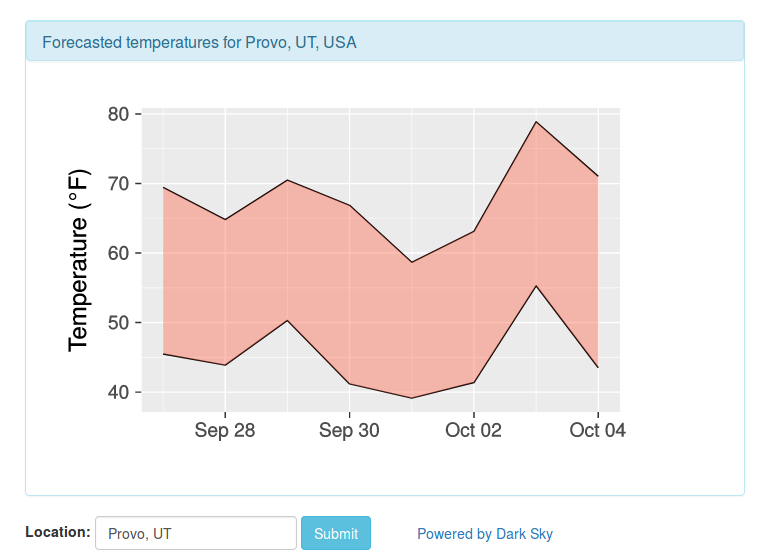
\includegraphics{screenshot.png}
\caption{Screenshot of a web application implemented in a \Scala-based
framework and accessing \R packages using \rscala.}
\label{screenshot}
\end{center}
\end{figure}

\pkg{Apache Spark}, a cluster-computing framework for massive datasets, is
another example of a \Scala application that might benefit from access to \R.
\pkg{Spark} provides an application programming interface to \Scala, \Java, \R,
and \Python.  \R users who are not already familiar with \Scala would be best
served by accessing \pkg{Spark} from \R using a dedicated package such as
\pkg{sparklyr} or \pkg{sparkr}.  \Scala developers, however, might prefer to
program directly with \pkg{Spark}'s Machine Learning Library (MLlib) in \Scala
and to supplement its functionality with \R through \rscala.  Recall that every
\code{RClient} has its own workspace, so several instances can be used to
overcome the single-threaded nature of \R.  One could, for example, use
\pkg{Apache Commons Pool} to manage a pool of \code{RClient} objects on each
worker node.  One potential limitation is the cost of pushing large datasets
over the TCP/IP bridge.

% We have provided support to a developer using \rscala in \pkg{Spark}.


% \subsection[Implementation of Scala code in R]{Implementation of \Scala code in \R}
% 
% The \code{scala} function starts a \Scala interpreter on the Java Virtual Machine using \R's
% \code{system2} function. The interpreter runs code that implements an asynchronous TCP/IP server
% and creates an instance of \code{scala.tools.nsc.interpreter.IMain} for \Scala's
% read-eval-print-loop (REPL). The TCP/IP
% server's port is randomly selected by default, but it can be fixed at a
% given value.  While the \Scala
% server is starting up, the \R component attempts to establish a connection using
% functions from the \pkg{base} \R package.  After connecting, the \R client interfaces with the
% server's REPL class by means of a custom protocol.
% 
% The \rscala package takes advantage of the \Scala REPL's ability to compile and
% execute \Scala code on-the-fly as well as set and get values of
% identifiers.  When a \Scala function is called for the first time (or when a
% particular method of a \Scala reference is called for the first time), it is
% compiled behind the scenes.  The compiled method is then
% cached and re-used for subsequent calls.  As an illustration, consider the code
% below and notice that the elapsed time is significantly less in the second call
% to the same method.
% 
% <<fasterAfterFirstTime>>=
% system.time( print(s$.sys$props("user.name")) )
% system.time( print(s$.sys$props("user.name")) )
% @
% 
% 
% 
% Callback functionality is implemented over the same TCP/IP sockets.
% Immediately after the \R client requests the execution of \Scala code, \R
% becomes a temporary, embedded server to allow the \Scala code to access the \R
% interpreter through the \code{R} object (an instance of the \code{RClient}
% class).  The embedded \R server interprets code and sets/gets values using the
% \code{parse}, \code{eval}, \code{assign}, and \code{get} functions.  After the
% \Scala server executes the \Scala code, it tells the embedded \R server to exit
% and the \Scala server resumes its usual behavior.

% \subsection{Bayesian logistic regression}
% \label{logisticRegression}
% 
% In this section we use a custom Markov chain Monte Carlo (MCMC) algorithm to
% fit a Bayesian logistic regression model in \R.  This model can also be
% estimated in \R through a variety of other algorithms using \R packages such as
% RStan \citep{stan-manual:2014}, rbugs \citep{Rbugs}, R2jags \citep{r2jags},
% rjags \citep{Rjags}, R2WinBUGS \citep{r2winbugs}, R2OpenBUGS
% \citep{r2openbugs}, and BRugs \citep{brugs}.  Our interest here,
% however, is \emph{not} to determine the best algorithm for Bayesian model
% fitting, but rather to compare the convenience and computational speed of
% \Scala, \C, and standard \R in implementing the same commonly-used,
% computationally-expensive algorithm.
% 
% Studies show that babies who breastfeed have a significantly reduced risk of
% health problems such as HIV, obesity, and neurological defects due to the
% fact that milk contains natural immune components that are not present in baby
% formula \citep{standby}.  Medical professionals have observed that premature
% babies take longer to learn how to breastfeed and many are not breastfeeding by
% the time they are ready to leave the hospital \citep{standby2}.  To quantify
% this relationship, a statistician wishes to fit a logistic regression model in
% which the probability of breastfeeding before leaving the hospital is modeled
% as a function of gestational age.  Data is available on $n=64$ infants where
% $y_i = 1$ if the baby is breastfeeding at departure and $x_i$ is the
% gestational age.  The model is
% \[
% \text{Pr}(y_i = 1) \ = \ \frac{1}{1+\exp\{-(\beta_0 + \beta_1 x_i)\}}
% \]
% where $\beta_0$ and $\beta_1$ are unknown parameters to estimate.  We assume
% independent Normal($-15$, $5$) and Normal($1$, $1$) priors on $\beta_0$ and
% $\beta_1$, respectively.
% 
% Since the model is not conjugate, we obtain samples from the joint posterior
% distribution using a Metropolis sampling algorithm with a uniform random walk.
% We examine the convenience and computational speed of running a single MCMC
% chain as well as simultaneously running 6 and 12 independent chains in
% parallel.  Recall that the test machine has 6 cores and hyperthreading is enabled
% making it appear that there are 12 cores.  We run the chains for 1,001,000
% iterations using the prior means as the starting state.  We discard the first
% 1,000 iterations for burn-in. This same MCMC algorithm is implemented in \Scala
% using \rscala, in \C using the \code{.C} interface, and in standard \R.  Note
% that a \C implementation using the \code{.Call} interface requires a more
% intimate knowledge of \R's \C API.  The implementations, data, and benchmarking
% code are all available in the online supplement.
% 
% \begin{table}[tb]
% \centering
% \begin{tabular}{r|rr|rr|rr}
%   \toprule
%  & \multicolumn{2}{c|}{1 core} & \multicolumn{2}{c|}{6 cores} & \multicolumn{2}{c}{12 cores} \\
% Language & Seconds & Ratio & Seconds & Ratio & Seconds & Ratio \\
%    \midrule
% \Scala using \rscala  & 1.12 & 1.00 & 0.29 & 1.00 & 0.18 & 1.00 \\
% \C using \code{.C}    & 1.48 & 1.32 & 0.31 & 1.09 & 0.24 & 1.36 \\
% Standard \R           & 15.79   & 14.11 & 3.78 & 13.15 & 2.70 & 15.08 \\
%    \bottomrule
% \end{tabular}
% \caption{Wall time and relative performance of three implementations of the same
% MCMC algorithm using 1, 6, and 12 cores based on a breastfeeding dataset with 64 samples and 6 levels of the predictor.}
% \label{mcmcInfant}
% \end{table}
% 
% The results are in Table~\ref{mcmcInfant} along with wall times and performance
% ratios (relative to \Scala).  Surprisingly, we find that the \Scala
% implementation is slightly faster than the \C implementation.  This may be due
% to the fact that the \Scala code uses a different library for evaluating the
% log of the binomial probabilities or because the \code{.C} interface is not as
% performant as the \code{.Call} interface.  The standard \R implementation is
% about 13-15 times slower.
% 
% The breastfeeding infants example involves $n=64$ observations at one of six
% unique values of the predictor.  To see how the results might change for larger
% datasets, we simulated a dataset of $n=20,000$ observations at one of 200
% unique values of the predictor.  The results are found in
% Table~\ref{mcmcSimulated}.  The most striking finding is that the standard \R
% implementation improves dramatically, now being only 1.4-1.6 times slower than
% the \Scala implementation.  The explanation is that the standard \R
% implementation, for this simulated data example, spends 72.5\% of the time in
% the function \code{dbinom}.  This function is implemented in \C using the
% \code{.Call} interface.  It is not surprising that a \C implementation
% and another implementation based mostly on \C (i.e., the standard \R
% implementation) perform similarly.
% 
% \begin{table}[tb]
% \centering
% \begin{tabular}{r|rr|rr|rr}
%   \toprule
%  & \multicolumn{2}{c|}{1 core} & \multicolumn{2}{c|}{6 cores} & \multicolumn{2}{c}{12 cores} \\
% Language & Seconds & Ratio & Seconds & Ratio & Seconds & Ratio \\
%    \midrule
% \Scala using \rscala  & 47.35 & 1.00 & 10.82 & 1.00 & 7.87 & 1.00 \\
% \C using \code{.C}    & 53.17 & 1.12 & 11.49 & 1.06 & 7.67 & 0.97 \\
% Standard \R           & 75.51 & 1.59 & 16.15 & 1.49 & 11.30 & 1.44 \\
%    \bottomrule
% \end{tabular}
% \caption{Wall time and relative performance of three implementations of the same MCMC
% algorithm using 1, 6, and 12 cores based on a simulated dataset with 20,000 samples and 200 levels of the predictor.}
% \label{mcmcSimulated}
% \end{table}

\section[Case study: Simulation study accelerated with rscala]{Case study: Simulation study accelerated with \rscala}
\label{bootstrap}

While the previously mentioned \pkg{shallot} and \pkg{bamboo} packages demonstrate the
ability to develop packages based on \rscala, we now demonstrate 
the ease with which computationally-intensive statistical procedures can be
implemented by embedding \Scala code in an \R script.  The algorithm is
embarrassingly parallel and we consider two means of parallelization: one using
\Scala's \code{Future} class and the other using \R's \pkg{parallel} package.
By way of comparison, we include a pure \R implementation of the same algorithm, 
and also an implementation that uses inline \Cpp code via the \Rcpp package. 
All four implementations define a
function that takes an \R sampling function as an argument.

We investigate a simulation study of the coverage probability of a bootstrap
confidence interval procedure.  Consider a population parameter
$\beta_1/\beta_2$, where $\beta_1$ and $\beta_2$ are population quantiles
associated with probabilities $p_1$ and $p_2$, respectively.  Based on a sample
of $n$ observations, a point estimator of the parameter is the ratio of the
corresponding sample quantiles and the following bootstrap procedure can be
used to find a confidence interval
when the population distribution is unspecified. The sample estimate is
recorded for each of \code{nSamples} bootstrap samples.  A bootstrap confidence
interval is given by $(l, u)$, where $l$ and $u$ are quantiles of the bootstrap
sampling distribution associated with $\alpha/2$ and $1-\alpha/2$,
respectively.  Although the nominal coverage is $1-\alpha$, interest lies in
computing the actual coverage probability of this bootstrap confidence interval
procedure using a Monte Carlo simulation study.  \code{nIntervals} samples from
the population are obtained from a user-supplied sampling function.  Although
the code is general, we sample $n=100$ observations from the standard normal
distribution and set $p_1=0.75$ and $p_2=0.35$, making $\beta_1/\beta_2 \approx
-1.75$.  We use \code{nIntervals} = 10,000 Monte Carlo replicates, each having
\code{nSamples} = 10,000 bootstrap samples.

The four implementations are available in the
Appendix, in the package, and at
{\footnotesize
\url{https://raw.githubusercontent.com/dbdahl/rscala/master/R/rscala/inst/doc/bootstrap-coverage.R}}.
The \R implementation is the shortest and the \rscala implementation
is somewhat more concise than the \Rcpp implementation.  The pure \R
iterates using apply functions.  The \Rcpp implementation is
written in \C style.  The pure \R, \Rcpp, and second \rscala implementations
use the \pkg{parallel} package to harness all available cores, whereas the
first \rscala implementation uses \Scala's \code{Future} class for parallelism.
In the first \rscala implementation, a single instance of \code{RClient} is
used by multiple JVM threads to call back to the single \R instance when
sampling the data.  On machines with many cores, having each thread wait its
turn to access the \R instance will likely slow down the execution.  In the
second \rscala implementation, each CPU core has a separate \R instance with a
corresponding \code{RClient}.

We tested on four machines running Ubuntu 16.04 with 8 cores, Ubuntu 16.04 with
56 cores, Mac Sierra with 8 cores, and Windows 10 with 8 cores.  \R was
compiled from source for the Ubuntu machines and was installed from binaries
downloaded from CRAN for the Mac and Windows machines.  All machines ran \R
3.4.1, \Scala 2.12.3, \Java 8, \Rcpp 0.12.12, and a prerelease version of
\rscala 2.3.1.

\begin{table}
\begin{center}
\begin{tabular}{c|lrrrrrr}
\toprule
Machine & Implementation&  Min.& $Q_1$&  Mean&Median& $Q_3$&   Max.\\
\midrule
\parbox[t]{4ex}{\multirow{4}{*}{\rotatebox[origin=c]{90}{\parbox{10ex}{\centering Ubuntu\\ 8 cores}}}}
   & Pure \R     & 1858.1 & 1863.9 & 1875.9 & 1867.9 & 1878.9 & 1943.8 \\
   & \Rcpp       &  105.1 &  105.3 &  107.3 &  105.6 &  106.5 &  118.6 \\
   & \rscala \#1 &   81.8 &   82.0 &   82.5 &   82.2 &   82.5 &   84.8 \\
   & \rscala \#2 &   70.2 &   70.4 &   71.4 &   70.7 &   70.9 &   77.9 \\
\midrule
\parbox[t]{4ex}{\multirow{4}{*}{\rotatebox[origin=c]{90}{\parbox{10ex}{\centering Ubuntu\\ 56 cores}}}}
  & Pure \R      &  444.1 &  449.8 &  450.8 &  451.3 &  452.4 &  456.1 \\
  & \Rcpp        &   19.7 &   19.6 &   19.7 &   19.8 &   19.8 &   20.0 \\
  & \rscala \#1  &   46.9 &   47.7 &   48.0 &   48.0 &   48.6 &   49.0 \\
  & \rscala \#2  &   14.5 &   14.6 &   16.6 &   14.8 &   15.0 &   32.2 \\
\midrule
\parbox[t]{4ex}{\multirow{4}{*}{\rotatebox[origin=c]{90}{\parbox{10ex}{\centering Mac\\ 8 cores}}}}
  & Pure \R      &        &        &        &        &        &        \\
  & \Rcpp        &  136.9 &  137.1 &  139.3 &  139.8 &  140.7 &  141.8 \\
  & \rscala \#1  &   93.4 &  94.2  &   94.7 &   94.9 &   95.3 &   95.8 \\
  & \rscala \#2  &   91.2 &  92.5  &   93.4 &   92.6 &   92.7 &  101.8 \\
\midrule
\parbox[t]{4ex}{\multirow{4}{*}{\rotatebox[origin=c]{90}{\parbox{10ex}{\centering Windows\\ 8 cores}}}}
  & Pure \R      &        &        &        &        &        &        \\
  & \Rcpp        &  184.8 &  185.0 &  187.6 &  185.3 &  186.1 &  201.8 \\
  & \rscala \#1  &  108.9 &  109.1 &  109.3 &  109.1 &  109.5 &  110.1 \\
  & \rscala \#2  &  106.7 &  107.3 &  107.8 &  107.9 &  108.0 &  109.9 \\
\bottomrule
\end{tabular}
\end{center}
\caption{Elapsed time (in seconds) for the four implementations of the
bootstrap simulation study executed on four different machines.  Overall, the
second \rscala implementation had the fastest execution times.}
\label{benchmarks}
\end{table}

Elapsed times (in seconds) for 10 replications of the simulation study are
found in Table \ref{benchmarks}.  For the sake of expediency, the pure \R
implementation was only run on the Ubuntu machines.  The pure \R implementation
ran more than 26 times slower than the fastest implementation.  The second
\rscala implementation (which uses the \pkg{parallel} package) was the fastest
overall.  The first \rscala implementation was close behind, except on the
Ubuntu machine with 56 cores, which illustrates the difficulty of sharing a
single \R instance across all of the cores.  The \Rcpp implementation is generally
slower than the \rscala implementations, but still much faster than
the pure \R implementation.

\section{Conclusion}
\label{conclusion}

This paper introduced the \rscala software to bridge \R and \Scala.  The
software allows a user to leverage their skills in both languages and to
utilize libraries and exploit strengths in each language.  For example, \R
users can implement computationally intensive algorithms in \Scala, write \R
packages based on \Scala, and access \Scala libraries from \R.  \Scala
programmers can take advantage of \R's tools for data analysis and graphics
from within a \Scala application. 

We are exploring two possible features to improve the package.  The first would
allow embedded \Scala computations to be interrupted by the \R user without
destroying the TCP/IP bridge.  The second feature would permit \R and \Scala to
run on separate machines.

\section*{Acknowledgements}

The author's work on this paper was supported by NIH NIGMS R01 GM104972.  The
author thanks the CRAN maintainers for their excellent service.  The author
also thanks the following students for valuable feedback on the software and
paper: Floid Gilbert, Brandon Carter, Deepthi Uppalapati, Scott Ferguson, and
Richard Payne.

\bibliography{refs}

\setcounter{section}{0}
\renewcommand{\thesection}{Appendix \Alph{section}}

\newpage
\section{}


{
\footnotesize
\VerbatimInput[numbers=left,xleftmargin=5mm]{../inst/doc/bootstrap-coverage.R}
}

\end{document}



